\chapter{Manifolds}

\begin{quote}
	{\color{orange} \textbf{Very important note:}} Throughout this text, to avoid repeating some words like \emph{smooth,  and etc}, we often omit them and we let the context to reflect these notions. So we emphasis that throughout this text, unless otherwise specified, by a \textbf{manifold} we always mean a $ C^\infty $ manifold. An atlas of a chart on a smooth manifold means an atlas or a chart contained in the differentiable structure of the smooth manifold.
\end{quote} 


\section{Topological manifolds and Smooth manifolds}

We start with the definition of topological manifolds. We will later study the smooth manifolds that are of our main interest in this lecture. But first, we need to review some basic definition.

\begin{definition}[Hausdorff topological space]
	A set $ A $, along with a collection of subsets of $ A $ called $ \mathcal{T} \subset 2^A $, i.e. $ (A,\mathcal{T}) $ is called a topological space if we have
	\begin{enumerate}[(I)]
		\item $ \emptyset \in \mathcal{T} $ and $ A \in \mathcal{T} $.
		\item For any infinite collection $ \set{A_\alpha}_\alpha \subset \mathcal{T} $ we have
		\[ \bigcup_{\alpha} A_\alpha \in \mathcal{T}. \]
		\item For a finite collection $ \set{A_i}_{i \in I} $ where $ I = \set{1,2,\cdots,N} $ for some $ N \in \N $, we have
		\[ \bigcap_{i \in I} A_i \in \mathcal{T}. \]
		\item $ \forall x,y \in A $ there exists $ U,V \in \mathcal{T} $ such that $ x\in U $ and $ y \in V $ and we have $ U \cap V = \emptyset $.
	\end{enumerate}
\end{definition}


The following definition reviews the notion of second countable topological spaces.

\begin{definition}[Second countable topological spaces]
	Let $ (X,\mathcal{T}) $ be a topological space. This space is second countable if there exists an at most countable collection of sets $ \mathcal{B} \subset \mathcal{T} $ such that $ \forall U \in \mathcal{T} $ we have
	\[ U = \bigcup_{A \in \mathcal{B}} A. \]
	I.e. any open set in $ \mathcal{T} $ can be written as a union of sets in $ \mathcal{B} $
\end{definition} 

The last piece of definition that we need is the notion of locally Euclidean spaces.

\begin{definition}[Locally Euclidean topological spaces]
	Let $ (X,\mathcal{T}) $ be a topological space. We say $ X $ is locally Euclidean if $ \forall p \in X $, there exists an open neighborhood $ p \in U \in \mathcal{T}$ such that is homeomorphic to an \emph{open} subset of $ \R^n $. I.e. there is a homeomorphism $ \phi: U \to \R^n $. We call the pair $ (U,\phi:U\to\R^n) $ a \emph{chart}, $ U $ a \emph{coordinate neighborhood} or a \textbf{coordinate open set}, and $ \phi $ a \emph{coordinate map} or \emph{coordinate system} on $ U $. 
\end{definition}


\begin{definition}[Topological manifolds]
	A topological manifold is a Hausdorff, second countable topological space that is locally Euclidean space. It is said to be of dimension $ n $, if it is locally Euclidean of dimension $ n $.
\end{definition}


In the following section, we will review the notion of compatible charts which will be central to our study of manifolds. Assume we have two charts $ (U,\phi) $ and $ (V,\psi) $. Since $  U,V $ are open in $ M $ (the manifold), then $ U\cap V $ is open in $ U $ and $ V $. Furthermore, since $ \phi $ is a homeomorphism to an open subset of $ \R^n $ then $ \phi(U\cap V) $ and $ \psi(U\cap V) $ are also open. One way to show this, let $ \phi(U cap V) = B, \phi(U) = A, $ and $ A\backslash B = C $. We know that $  A $ is open, and $ B\cup C = A, B \cap C = \emptyset $. Then $ A $ being open implies $ B $ and $ C $ is open. Now we can make the following definition for $ C^\infty $-compatible maps.

\begin{definition}[$ C^\infty $ compatible maps]
	Let $ M $ be a topological manifold, where $ (U,\phi) $ and $ (V,\psi) $ are two charts. These charts are called $ C^\infty $-compatible if the maps
	\[ \phi\circ \inv{\psi} : \psi(U\cap V) \to \phi(U\cap V)\qquad \text{and} \qquad  \psi \circ\inv{\phi}: \phi(U \cap V) \to \psi(U\cap V),  \]
	are $ C^\infty $. These two maps are called \emph{transition functions} between charts. 
\end{definition}

\begin{remark}
	If two $ U,V $ in the definition above, i.e. $ U\cap V = \emptyset $, then they are automatically compatible.
\end{remark}

\begin{definition}[$ C^\infty $ atlas]
	Let $ M $ be a topological manifold. The collection of charts $ \mathcal{U} = \set{(U_\alpha, \phi_\alpha)} $ is called a $ C^\infty $ atlas, or simply an atlas if 
	\begin{itemize}
		\item all of the charts are pairwise $ C^\infty $ compatible,
		\item the charts cover the whole manifold, i.e. $ M = \bigcup_\alpha U_\alpha $.
	\end{itemize}
\end{definition}

\begin{lemma}
	Let $ \mathcal{A} = \set{(U_\alpha,\phi_\alpha)}_{\alpha \in I} $ be an atlas for the manifold $ M $. Let $ (V,\psi) $ and $ (W,\sigma) $ be two charts where both of them are compatible with the atlas $ \mathcal{A} $. Then these two charts are compatible with each other.
\end{lemma}

\begin{proof}
	We start by showing that $ \psi\circ \inv{\sigma} $ is $ C^\infty $ on $ V\cap W $. Let $ p \in V \cap W $. Then $ \exists \alpha \in I $ such that $ p \in U_\alpha $ for the chart $ (U_\alpha,\phi_\alpha) $. Then 
	\[ (\psi \circ \inv{\phi_\alpha})\circ (\phi_\alpha \circ \inv{\sigma}): \sigma(W\cap U_\alpha \cap V) \to \psi(W \cap U_\alpha \cap V) \]
	is $ C^\infty $ in $ \sigma(W\cap U_\alpha \cap V) $, because it is the composition of $ C^\infty $ maps. Call $ \mathbb{B}_\alpha  = W\cap U_\alpha \cap V $. Then what we have shows is simply $ \forall p \in V \cap W $, there exists an open set $ p \in \mathbb{B}_\alpha \subset V\cap W $ for $  \alpha \in I $ and the map $ \psi \circ \inv{\sigma}  $ is $ C^\infty $ in $ \mathbb{B}_\alpha $. Since this holds for every $ p \in V \cap W $ this proves that $ \psi\circ \inv{\sigma} $ is $ C^\infty $ on $ \sigma (V\cap W) $. Similarly, we can show $ \sigma \circ \inv{\psi} $ is $ C^\infty $ on $ \psi(V\cap W) $, and this completes the proof.
\end{proof}

\begin{remark}
	Note that in an equality like $ \psi \circ \inv{\sigma} =(\psi \circ \inv{\phi_\alpha})\circ (\phi_\alpha \circ \inv{\sigma}) $, two functions in the sides of the equality have different domains. So the equality sign here means that these two functions are equal on their common domain.
\end{remark}


\begin{definition}[Maximal atlas]
	Let $ \mathcal{U} $ be an atlas for the manifold $ M $. Then $ \mathcal{U} $ is called maximal if it contains any other atlas of the manifold $ M $. Or equivalently, if $ \mathcal{M} $ is any other atlas containing $ \mathcal{U} $ then $ \mathcal{U} = \mathcal{M} $.
\end{definition}

We can use the notion of the maximal atlas to define a smooth manifold.

\begin{definition}[Smooth manifold]
	A topological manifold together with a maximal atlas is called a smooth manifold. The maximal atlas is also called a differentiable structure on $ M $.
\end{definition}


In practice, to show that a topological manifold is smooth, it is not necessary to exhibit a maximal atlas. Existence of any atlas will do so, as proposed by the following proposition.


\begin{proposition}
	Any atlas of a locally euclidean space is contained in a \emph{unique} maximal atlas.
\end{proposition}

\begin{proof}
	Let $ \frak{U} = \set{(U_\alpha, \phi_\alpha)} $ be any atlas for the locally Euclidean space $ M $. Let $ S = \set{(V_i, \psi_i)} $ denote the set of all charts compatible with $ \frak{U} $. Construct the set $ \frak{M} = \frak{U} \cup S $. We claim that this set is a maximal atlas. Let $ (W,\psi) $ be a chart compatible with $ \frak{M} $. Then it should also be compatible with $ \frak{U} $, thus it is contained in the set $ S $, i.e. $ (W,\psi) \in S $, thus in $ \frak{M} $. This shows that the atlas $ \frak{M} $ is maximal.
	
	To show the uniqueness, let $ \frak{M}' $ be another maximal atlas. Since $ \frak{M}' $ is compatible with $ \frak{U} $, thus it is also compatible with $ \frak{M} $. But due to the construction it is contained in the new atlas, thus $ \frak{M}' \subset \frak{M} $. Thus the maximal atlas is unique.
\end{proof}

Considering the proposition above, we arrive at the following important observation.

\begin{observation}[Showing a space is an smooth manifold]
	To show that a space is an smooth manifold, we just need to show that the space is
	\begin{itemize}
		\item a Hausdorff topological space that is also second countable,
		\item there exists any $ C^\infty $ atlas (not necessarily maximal).
	\end{itemize}
\end{observation}


\section{Smooth maps on a manifold}
In this section, we will study the notion of smooth maps between manifolds. We will use the notion of coordinate charts to transfer the notion of smooth maps from Euclidean spaces to manifolds. We start with the functions on manifolds.

\begin{definition}[Smooth functions on manifolds]
	Let $ f:M \to R $ be a function on a manifold. The function $ f $ is smooth at point $ p \in M $ if there exists a chart $ (U,\phi) $ such that $ p \in U $ and the map
	\[ f \circ \inv{\phi}\ :\ \phi(U) \to \R \]
	is smooth at $ p $. The function $ f $ is said to be $ C^\infty $ on $ M $ if it is $ C^\infty $ at every point of $ M $.
\end{definition}
\begin{remark} 
	Note that the smoothness of the function $ f $ in the definition above is independent of the local chart $ (U,\psi) $ that we choose. Let $ (V,\psi) $ be another local chart containing the point $ p $. Then the map $ f \circ \inv{\psi} $ is also smooth at $ p $. Because
	\[ f \circ \inv{\psi}: (f\circ \inv{\phi}) \circ (\phi \circ \inv{\psi}). \]
	We know that the map $ (\phi \circ \inv{\psi} $ is smooth at $ p $ (since the local charts in an atlas are compatible). Also $ (f\circ \inv{\phi}) $ is smooth (we have assumed so). Thus $ f \circ \inv{\psi} $ is smooth.
\end{remark}

\begin{proposition}[Smoothness of real valued functions]
	Let $ M $ be a manifold of dimension $ n $ with atlas $ \frak{U} $, and let $ f: M \to \R $ a real-valued function on $ M $. The following are equivalent:
	\begin{enumerate}[(i)]
		\item The function $ f : M \to \R $ is $ C^\infty $.
		\item The manifold $ M $ has an atlas such that for every chart $ (U,\phi) $ in the atlas, $ f\circ \inv{\phi}: \phi(U) \to \R$ is $ C^\infty $.
		\item For every chart $ (V,\psi) $ on $ M $, the function $ f\circ \inv{\psi}: \psi(V) \to \R $ is $ C^\infty $.
	\end{enumerate}
\end{proposition}

\begin{proof}
	We prove a cyclic chain of implications $ (ii)\implies (i) \implies (iii) \implies (ii) $.
	
	\noindent $ (ii) \implies (i) $: Let $ p \in M $. From the assumption we know that there is an atlas with the desired property. Thus $ \exists (U_\alpha,\phi_\alpha)  $ that contains $ p $ and the function $ f\circ\inv{\phi}: \phi(U) \to \R $ is smooth. 
	Thus $ f:M\to \R $ is smooth at $ p $, ans since the point $ p $ was arbitrary, then $ f $ is smooth on $ M $.
	
	\noindent $ (i) \implies (iii) $: Let $ p \in U $. From assumption we know that there is a coordinate open set $ U_\alpha $ such that $ f \circ \inv{\phi_\alpha}: \phi_\alpha(U)\to \R $ is smooth. Then we can write
	\[ f\circ\inv{\psi} = (f\circ\inv{\phi_\alpha})\circ(\phi_\alpha \circ \inv{\psi}) \]
	which shows that $ f\circ\inv{\psi}  $ is smooth (look at the remark below).
	
	\noindent $ (iii) \implies (ii) $: This follows immediately from the definition.
\end{proof}

%\begin{quote}
%	{\color{orange} I am not sure about the remark below. I need to discuss this with Ata in one of our weekly meetings$\ \Downarrow\Downarrow\Downarrow\Downarrow$.}
%\end{quote}
%\begin{remark}
%	Note that when we are saying ``let $ M $ be a manifold of dimension $ n $'' (in the first part of the proposition), what we really means is that the set $ M $ along with the collection of compatible charts (i.e. atlas) $ \frak{U} $ forms a manifold. In the part (iii) of the proposition above, when we say ``for every chart $ (V,\phi) $'' on manifold $ M $, what we really mean is $ (V,\phi) $ is compatible with $ \frak{U} $.
%\end{remark}

\begin{remark}
	Considering the ``very important note'' at the beginning of this chapter, we need to emphasis again that in part $ (iii) $, when we say \emph{for every chart $ (V,\psi) $ on $ M $}, we mean a chart in the unique differentiable structure of the manifold that contains the atlas $ \frak{U} $.
\end{remark}

\begin{observation}[From W. Tu]
	The smoothness conditions from the proposition above will be a recurrent motif through out the book. To prove the smoothness of an object, it is sufficient that a smoothness criterion hold on the charts of some atlas. Once the object is shown to be smooth, it then follows that the same smoothness criterion holds on every chart on the manifold.
\end{observation}


\begin{definition}[Pull back of a function]
	Let $ F: N\to M $ be a a map between manifolds, and $ \phi: M \to \R $. Then the pullback of the function $ \phi $ by $ F $ is denoted by $ F*\phi $ is defined as 
	\[ F^* \phi = \phi\circ F. \]
\end{definition}

\begin{remark}
	In this terminology, a function $ f:M \to \R $ is smooth on a chart $ (U,\phi) $ if and only if the pullback $ (\inv{\phi})^* f$ is smooth on the subset $ \phi(U) $ of Euclidean space.
\end{remark}

\subsection{Smooth maps between manifolds}
Here in this section we will discuss the smooth maps between manifolds. We will be able to recover the definition of the smooth functions on manifolds as a special case. 

\begin{definition}[Smooth maps between manifolds]
	Let $ M, N $ be manifolds with dimensions $ m,n $ respectively. A map $ F: M \to N $ is said to be smooth at point $ p \in M $, if there exists charts $ (U,\phi) $ and $ (V,\psi) $ such that $ p \in U $ and $ F(p) \in V $, and the function 
	\[ \psi\circ F \circ \inv{\phi}: \R^m \supset \phi(\inv{F}(V) \cup U) \to \R^n  \]
	is smooth at $ p $. The map $ F $ is said to be smooth on manifold $ M $ if it is smooth at every point of the manifold.
\end{definition}
\begin{remark}
	The following figure helps to digest the definition above.
	\begin{figure}[h!]
	\centering
	
	
	
	
	
	\tikzset{every picture/.style={line width=0.75pt}} %set default line width to 0.75pt        
	
	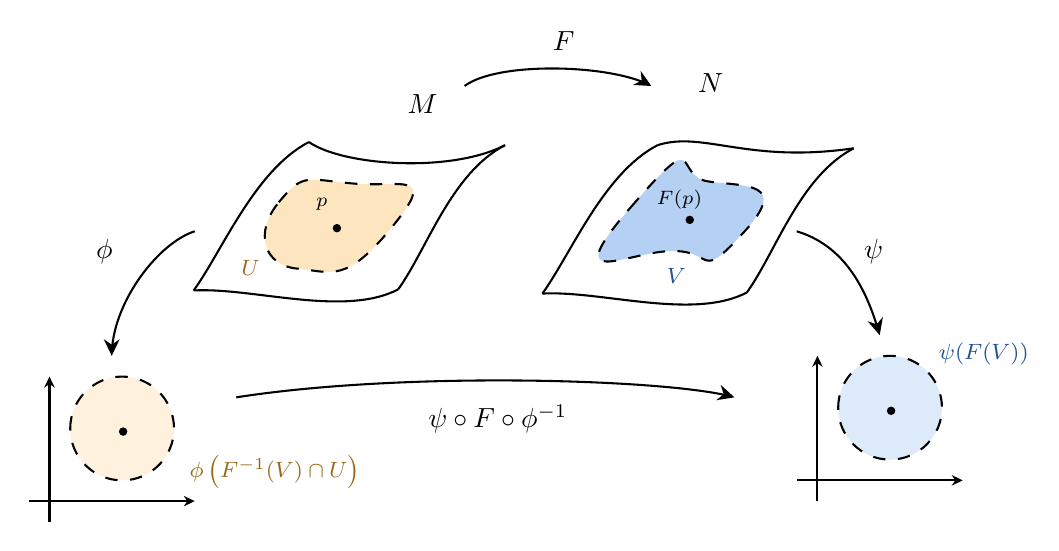
\begin{tikzpicture}[x=0.75pt,y=0.75pt,yscale=-1,xscale=1]
		%uncomment if require: \path (0,300); %set diagram left start at 0, and has height of 300
		
		%Curve Lines [id:da11806081372332144] 
		\draw    (179.5,178.5) .. controls (193.5,159) and (209,120.5) .. (235,107) ;
		%Curve Lines [id:da18965221151827483] 
		\draw    (179.5,178.5) .. controls (208,177) and (252,191.5) .. (278,178) ;
		%Curve Lines [id:da4778597706036809] 
		\draw    (278,178) .. controls (292,158.5) and (303.5,122) .. (329.5,108.5) ;
		%Curve Lines [id:da40033578881982557] 
		\draw    (235,107) .. controls (251.5,118.5) and (303.5,122) .. (329.5,108.5) ;
		%Curve Lines [id:da8289769291382043] 
		\draw    (347.5,180) .. controls (361.5,160.5) and (377,122) .. (403,108.5) ;
		%Curve Lines [id:da562782587348567] 
		\draw    (347.5,180) .. controls (376,178.5) and (420,193) .. (446,179.5) ;
		%Curve Lines [id:da8325596531064072] 
		\draw    (446,179.5) .. controls (460,160) and (471.5,123.5) .. (497.5,110) ;
		%Curve Lines [id:da2852542457229288] 
		\draw    (403,108.5) .. controls (425,101.5) and (446.5,117.5) .. (497.5,110) ;
		%Shape: Polygon Curved [id:ds40810252904164956] 
		\draw  [fill={rgb, 255:red, 245; green, 166; blue, 35 }  ,fill opacity=0.29 ][dash pattern={on 4.5pt off 4.5pt}] (220.5,136) .. controls (232.5,121.5) and (233.5,125) .. (256.5,127) .. controls (279.5,129) and (297.5,120.5) .. (275,148) .. controls (252.5,175.5) and (246,169.5) .. (229.5,168) .. controls (213,166.5) and (208.5,150.5) .. (220.5,136) -- cycle ;
		%Shape: Polygon Curved [id:ds4832622018481927] 
		\draw  [fill={rgb, 255:red, 74; green, 144; blue, 226 }  ,fill opacity=0.41 ][dash pattern={on 4.5pt off 4.5pt}] (390,138.5) .. controls (425.5,97.5) and (410,123.5) .. (427.5,126) .. controls (445,128.5) and (467,126) .. (444.5,150.5) .. controls (422,175) and (431,159) .. (409.5,159.5) .. controls (388,160) and (354.5,179.5) .. (390,138.5) -- cycle ;
		%Straight Lines [id:da8425805433734557] 
		\draw    (110,223) -- (110,290) ;
		\draw [shift={(110,220)}, rotate = 90] [fill={rgb, 255:red, 0; green, 0; blue, 0 }  ][line width=0.08]  [draw opacity=0] (5.36,-2.57) -- (0,0) -- (5.36,2.57) -- (3.56,0) -- cycle    ;
		%Straight Lines [id:da3867027047624212] 
		\draw    (177,280) -- (100,280) ;
		\draw [shift={(180,280)}, rotate = 180] [fill={rgb, 255:red, 0; green, 0; blue, 0 }  ][line width=0.08]  [draw opacity=0] (5.36,-2.57) -- (0,0) -- (5.36,2.57) -- (3.56,0) -- cycle    ;
		%Shape: Circle [id:dp9021706695013989] 
		\draw  [fill={rgb, 255:red, 245; green, 166; blue, 35 }  ,fill opacity=0.15 ][dash pattern={on 4.5pt off 4.5pt}] (120,245) .. controls (120,231.19) and (131.19,220) .. (145,220) .. controls (158.81,220) and (170,231.19) .. (170,245) .. controls (170,258.81) and (158.81,270) .. (145,270) .. controls (131.19,270) and (120,258.81) .. (120,245) -- cycle ;
		%Straight Lines [id:da20897051537256983] 
		\draw    (480,213) -- (480,280) ;
		\draw [shift={(480,210)}, rotate = 90] [fill={rgb, 255:red, 0; green, 0; blue, 0 }  ][line width=0.08]  [draw opacity=0] (5.36,-2.57) -- (0,0) -- (5.36,2.57) -- (3.56,0) -- cycle    ;
		%Straight Lines [id:da4413765041127402] 
		\draw    (547,270) -- (470,270) ;
		\draw [shift={(550,270)}, rotate = 180] [fill={rgb, 255:red, 0; green, 0; blue, 0 }  ][line width=0.08]  [draw opacity=0] (5.36,-2.57) -- (0,0) -- (5.36,2.57) -- (3.56,0) -- cycle    ;
		%Shape: Circle [id:dp2483574720488635] 
		\draw  [fill={rgb, 255:red, 74; green, 144; blue, 226 }  ,fill opacity=0.19 ][dash pattern={on 4.5pt off 4.5pt}] (490,235) .. controls (490,221.19) and (501.19,210) .. (515,210) .. controls (528.81,210) and (540,221.19) .. (540,235) .. controls (540,248.81) and (528.81,260) .. (515,260) .. controls (501.19,260) and (490,248.81) .. (490,235) -- cycle ;
		%Curve Lines [id:da8553312339361681] 
		\draw    (310,80) .. controls (325.36,68.48) and (376.66,69.4) .. (397.55,78.78) ;
		\draw [shift={(400,80)}, rotate = 208.93] [fill={rgb, 255:red, 0; green, 0; blue, 0 }  ][line width=0.08]  [draw opacity=0] (8.04,-3.86) -- (0,0) -- (8.04,3.86) -- (5.34,0) -- cycle    ;
		%Curve Lines [id:da778090429217146] 
		\draw    (470,150) .. controls (490.75,156.27) and (502.18,173.72) .. (509.25,197.4) ;
		\draw [shift={(510,200)}, rotate = 254.36] [fill={rgb, 255:red, 0; green, 0; blue, 0 }  ][line width=0.08]  [draw opacity=0] (8.04,-3.86) -- (0,0) -- (8.04,3.86) -- (5.34,0) -- cycle    ;
		%Curve Lines [id:da210913418624189] 
		\draw    (180,150) .. controls (163.11,155.31) and (141.57,182.5) .. (140.08,207.31) ;
		\draw [shift={(140,210)}, rotate = 270] [fill={rgb, 255:red, 0; green, 0; blue, 0 }  ][line width=0.08]  [draw opacity=0] (8.04,-3.86) -- (0,0) -- (8.04,3.86) -- (5.34,0) -- cycle    ;
		%Curve Lines [id:da8925336292700183] 
		\draw    (200,230) .. controls (281,217.39) and (403.86,221.25) .. (437.17,229.25) ;
		\draw [shift={(440,230)}, rotate = 196.61] [fill={rgb, 255:red, 0; green, 0; blue, 0 }  ][line width=0.08]  [draw opacity=0] (8.04,-3.86) -- (0,0) -- (8.04,3.86) -- (5.34,0) -- cycle    ;
		%Shape: Circle [id:dp7473837647062398] 
		\draw  [fill={rgb, 255:red, 0; green, 0; blue, 0 }  ,fill opacity=1 ] (247,148.5) .. controls (247,147.67) and (247.67,147) .. (248.5,147) .. controls (249.33,147) and (250,147.67) .. (250,148.5) .. controls (250,149.33) and (249.33,150) .. (248.5,150) .. controls (247.67,150) and (247,149.33) .. (247,148.5) -- cycle ;
		%Shape: Circle [id:dp9244279482747275] 
		\draw  [fill={rgb, 255:red, 0; green, 0; blue, 0 }  ,fill opacity=1 ] (417,144.5) .. controls (417,143.67) and (417.67,143) .. (418.5,143) .. controls (419.33,143) and (420,143.67) .. (420,144.5) .. controls (420,145.33) and (419.33,146) .. (418.5,146) .. controls (417.67,146) and (417,145.33) .. (417,144.5) -- cycle ;
		%Shape: Circle [id:dp5699925804076371] 
		\draw  [fill={rgb, 255:red, 0; green, 0; blue, 0 }  ,fill opacity=1 ] (144,246.5) .. controls (144,245.67) and (144.67,245) .. (145.5,245) .. controls (146.33,245) and (147,245.67) .. (147,246.5) .. controls (147,247.33) and (146.33,248) .. (145.5,248) .. controls (144.67,248) and (144,247.33) .. (144,246.5) -- cycle ;
		%Shape: Circle [id:dp11209906657188418] 
		\draw  [fill={rgb, 255:red, 0; green, 0; blue, 0 }  ,fill opacity=1 ] (514,236.5) .. controls (514,235.67) and (514.67,235) .. (515.5,235) .. controls (516.33,235) and (517,235.67) .. (517,236.5) .. controls (517,237.33) and (516.33,238) .. (515.5,238) .. controls (514.67,238) and (514,237.33) .. (514,236.5) -- cycle ;
		
		% Text Node
		\draw (281,82.4) node [anchor=north west][inner sep=0.75pt]    {$M$};
		% Text Node
		\draw (421,72.4) node [anchor=north west][inner sep=0.75pt]    {$N$};
		% Text Node
		\draw (351,52.4) node [anchor=north west][inner sep=0.75pt]    {$F$};
		% Text Node
		\draw (501,152.4) node [anchor=north west][inner sep=0.75pt]    {$\psi $};
		% Text Node
		\draw (131,152.4) node [anchor=north west][inner sep=0.75pt]    {$\phi $};
		% Text Node
		\draw (291,232.4) node [anchor=north west][inner sep=0.75pt]    {$\psi \circ F\circ \phi ^{-1}$};
		% Text Node
		\draw (237,132.4) node [anchor=north west][inner sep=0.75pt]  [font=\scriptsize]  {$p$};
		% Text Node
		\draw (401,128.4) node [anchor=north west][inner sep=0.75pt]  [font=\scriptsize]  {$F( p)$};
		% Text Node
		\draw (201,162.4) node [anchor=north west][inner sep=0.75pt]  [font=\footnotesize,color={rgb, 255:red, 155; green, 104; blue, 25 }  ,opacity=1 ]  {$U$};
		% Text Node
		\draw (406,166.4) node [anchor=north west][inner sep=0.75pt]  [font=\footnotesize,color={rgb, 255:red, 29; green, 81; blue, 148 }  ,opacity=1 ]  {$V$};
		% Text Node
		\draw (537,202.4) node [anchor=north west][inner sep=0.75pt]  [font=\footnotesize,color={rgb, 255:red, 29; green, 81; blue, 148 }  ,opacity=1 ]  {$\psi ( F( V))$};
		% Text Node
		\draw (176,256.4) node [anchor=north west][inner sep=0.75pt]  [font=\footnotesize,color={rgb, 255:red, 155; green, 104; blue, 25 }  ,opacity=1 ]  {$\phi \left( F^{-1}( V) \cap U\right)$};
		
		
	\end{tikzpicture}
\end{figure}
\end{remark}

\begin{remark}
	Since the Euclidean space is indeed a smooth manifolds, then we can recover the definition of smooth functions on manifolds form the definition above. Let $ M $ be a manifold, and $ N = \R^n $ with the atlas $ \set{(\R^n, \mathds{1}: \R^n \to \R^n)} $, then we will have the notion of vector valued functions on manifold. By setting $ n=1 $ we will recover the definition of smooth function on manifold.
\end{remark}

In the following proposition we will be showing that the smoothness of the map is independent of the charts chosen, thus the smoothness of the map is well-defined.

\begin{proposition}[Smoothness of maps between manifolds is well-defined]
	\label{prop:SmoothnessWellDefined}
	Suppose $ F: N \to M $ is $ C^\infty $ at $ p \in N $. If $ (U,\phi) $ is any chart in $ N $ that contains $ p $ and $ (V,\psi) $ is any chart in $ M $ that contains $ F(p) $, then $ \psi \circ F \circ \inv{\phi} $ is smooth at $ \phi(p) $.
\end{proposition}

\begin{proof}
	Since $ F: N \to M $ is smooth at $ p \in N $, then there are charts $ (G,\gamma) $ and $ (L, \lambda) $ (from the corresponding maximal atlases) such that $ p \in G \subset N $ and $ F(p) \in L \subset M $ and the function 
	\[ (\lambda \circ F \circ \inv{\gamma}): \gamma(\inv{F}(L) \cap G ) \to \lambda(F(G)) \]
	is smooth at $ p $. Consider the charts $ (U,\phi) $ and $ (V,\psi) $ as above. Then the function
	\[ \psi \circ F \circ \inv{\phi} = (\psi \circ \inv{\lambda})\circ(\lambda\circ F \circ \inv{\gamma})\circ(\gamma\circ \inv{\phi}). \]
	Note that the equality sign above merely means the functions are equal on their common domain, as the function in RHS and the function in LHS have different domains. We know that the coordinate maps $ \psi, \lambda $, and $ \gamma, \phi$ are compatible respectively. Thus the function $ \psi \circ F \circ \inv{\phi} $ is smooth at $ \phi(p) $. See the remark below for mode details.
\end{proof}

\begin{remark}
	In the proof above and in the equality 
	\[ \psi \circ F \circ \inv{\phi} = (\psi \circ \inv{\lambda})\circ(\lambda\circ F \circ \inv{\gamma})\circ(\gamma\circ \inv{\phi}) \]
	thus equality sign does not indicate that these function are equal, but it just indicates that these two functions are equal in their common domain. To be more clear, for the function in the LHS we have
	\[ \psi \circ F \circ \inv{\phi} : \phi(\inv{F}(V)\cap U) \to \psi(F(U)). \]
	But for the function in the LHS we have
	\[ (\psi \circ \inv{\lambda})\circ(\lambda\circ F \circ \inv{\gamma})\circ(\gamma\circ \inv{\phi}):
	\phi(\inv{F}(L\cap V) \cap (G\cap U)) \to \psi(F(L\cap V))
	 \]
\end{remark}

\begin{proposition}[Smoothness of maps in terms of charts]
	\label{prop:smoothnessInTermsOfCharts}
	Let $ N $ and $ M $ be smooth manifolds, and $ F: N \to M $ a continuous map. The following are equivalent:
	\begin{enumerate}[(i)]
		\item The map $ F: N\to M $ is $ C^\infty $.
		\item There are atlases $ \frak{U} $ for $ N $ and $ \frak{V} $  for $ M $ such that for every chart $ (U,\phi) $ in $ \frak{U} $ and $ (V,\psi) $ in $ \frak{V} $ the map
		\[ \psi \circ F \circ \inv{\phi}: \phi(\inv{F}(V)\cap U) \to \R^m  \]
		is $ C^\infty $.
		\item For every chart $ (U,\phi) $ on $ N $ and $ (V,\psi) $ on $ M $, the map
		\[ \psi \circ F \circ \inv{\phi}: \phi(U \cap \inv{F}(V)) \to \R^m \]
		is $ C^\infty $.
	\end{enumerate}
\end{proposition}
\begin{proof}
	We will prove this by showing a cyclic chain of implications $ (ii)\implies (i)\implies (iii)\implies (ii) $.
	\begin{itemize}
		\item $ (ii)\implies (i) $. Let $ p \in N $. Then by hypothesis there are charts $ (U,\phi) $ and $ (V,\psi) $  such that $ p \in U $ and $ F(p) \in V $ and the map 
		\[ \psi \circ F \circ \inv{\phi}: \phi(\inv{F}(V)\cap U) \to \R^m \]
		is smooth at $ \phi(p) $, thus $ F $ is smooth at $ p $. Since $ p $ is arbitrary, then $ F $ is smooth on $ N $.
		\item $ (i) \implies (iii) $. This follows immediately from \autoref{prop:SmoothnessWellDefined}.
		\item $ (iii) \implies (ii) $. Since $ N, M $ are smooth manifolds, then they have maximal atlases. Let $ \frak{U} $ be the maximal atlas for $ N $ and $ \frak{V} $ be the maximal atlas for $ M $. This $ (ii) $ follows immediately form $ (iii) $.
		
	\end{itemize}
\end{proof}

\begin{proposition}[Composition of $ C^\infty $ maps]
	If $ F:N\to M $ and $ G:M\to P $ are $ C^\infty $ maps of manifolds, then the composite $ G\circ F: N \to P $ is a smooth map.
\end{proposition}

\begin{proof}
	We will demonstrate two proofs for this proposition to demonstrate what happens if we do not notice a possible level of abstraction. The first proof below is a very crude, hard-core, direct proof, that seems to be tough and easy to make mistakes, just because it is not encapsulating some of the details into another proposition. However, for the second proof, it will encapsulate some of the details into the results of the \autoref{prop:smoothnessInTermsOfCharts}, which will allows us to do a more high level thinking.
	
	\textbf{proof 1.} Let $ p \in M $. Since $ F $ is smooth, then $ \exists\ (U,\gamma) $ chart for $ M $ and $ \exists\ (V,\phi) $ chart for $ M $ such that $ p \in U $ and $ F(p) \in V $ and the map
	\[ \phi\circ  F \circ \inv{\gamma}: \gamma(\inv{F}(V)\cap U) \to \phi(V)  \]
	is smooth at $ \gamma(p) $. Also, since $ G $ is smooth, then at $ F(p) $, there exists the charts $ (W,\lambda) $ for $ M $ and $ (Y,\psi) $ for $ P $ such that $ F(p) \in W $ and $ G(F(p)) \in Y $ and the map
	\[ \psi\circ G \circ \inv{\lambda}: \lambda(\inv{G}(Y)\cap W) \to \psi(Y)  \]
	is smooth at $ \lambda(F(p)) $. Also note that since the charts $ (W,\lambda) $ and $ (V,\phi) $ for $ M $ are compatible (they both are chosen from the maxima atlas), then the maps
	\[ \phi \circ \inv{\lambda}: \lambda(W\cap V) \to \phi(W\cap V) \quad \text{and}\ \quad \lambda\circ \inv{\phi}:\phi(W\cap V) \to \lambda(W\cap V) \]
	are both smooth. Now it is time to glue all of these pieces together to infer the smoothness of the composite function $ G\circ F $. Based on these pieces, the function
	\[ \psi \circ (G \circ F) \circ \inv{\gamma} = ( \psi\circ G \circ \inv{\lambda})\circ (\lambda \circ \inv{\phi}) \circ (\phi\circ  F \circ \inv{\gamma}) : \gamma(\inv{F}(\inv{G}(Y)\cap V\cap W)\cap U)\to \psi(G(F(p))) \]
	is smooth at $ \gamma(p) $. Since the point $ p \in N $ was arbitrary, then the map $ G\circ F $ is smooth on $ M $.
	
	\textbf{proof 2.} In this proof, we will hide much of the details of the proof 1 in higher level of abstractions encapsulated in \autoref{prop:smoothnessInTermsOfCharts}.  Since $ F $ is smooth, then ($ (i)\implies (iii) $ of \autoref{prop:smoothnessInTermsOfCharts}) for every chart $ (U,\gamma) $  for $ M $ and $ (V,\phi) $  for $ M $ the map
	\[ \phi\circ  F \circ \inv{\gamma}: \gamma(\inv{F}(V)\cap U) \to \phi(V)  \]
	is smooth.. Also, since $ G $ is smooth, then for every chart  $(Y,\psi) $ for $ P $ the map
	\[ \psi \circ G \circ \inv{\phi}: \phi(\inv{G}(Y)\cap V) \to \psi(Y)  \]
	is smooth. Since the composition of smooth real vector valued functions is smooth, then 
	\[ \psi\circ(G\circ F)\circ\inv{\gamma} = (\psi\circ G\circ \inv{\phi})\circ(\phi \circ F \circ \inv{\gamma}) \]
	is smooth. Since for every chart $ (U,\gamma) $ and $ (Y,\phi) $ the function $ \psi\circ(G\circ F)\circ\inv{\gamma} $ is smooth, then by $ (iii)\implies (i) $ of \autoref{prop:smoothnessInTermsOfCharts} we proved that $G\circ F $ is smooth.
\end{proof}


\section{Diffeomorphisms}
We start with the definition of diffeomorphism.

\begin{proposition}[Diffeomorphism between manifolds]
	A map $ F:M\to N $ between manifolds $ M $ and $ N $ is called a diffeomorphism if
	\begin{itemize}[nosep]
		\item $ F $ is a bijection,
		\item $ F $ is $ C^\infty $, and
		\item $ \inv{F} $ is also $ C^\infty $.
	\end{itemize}
\end{proposition}

The following observation box summarizes the differences between homeomorphisms and diffeomorphisms.

\begin{observation}[Difference between homeomorphisms and diffeomorphisms]
	homeomorphisms are isomorphisms in the category of topological spaces. However, the diffeomorphisms are isomorphisms in the category of smooth manifolds, where the isomorphism preserves the differential structures. The following figure (original idea from\footnote{\href{https://www.math.unipd.it/~maraston/An2Byaounde/An2BCam_1213_1_mfds.pdf}{ mathematical analysis lecture notes.}}) demonstrates some of these ideas.
\end{observation}
	\begin{figure}[h!]
	\centering
	
	
	
	\tikzset{every picture/.style={line width=0.75pt}} %set default line width to 0.75pt        
	
	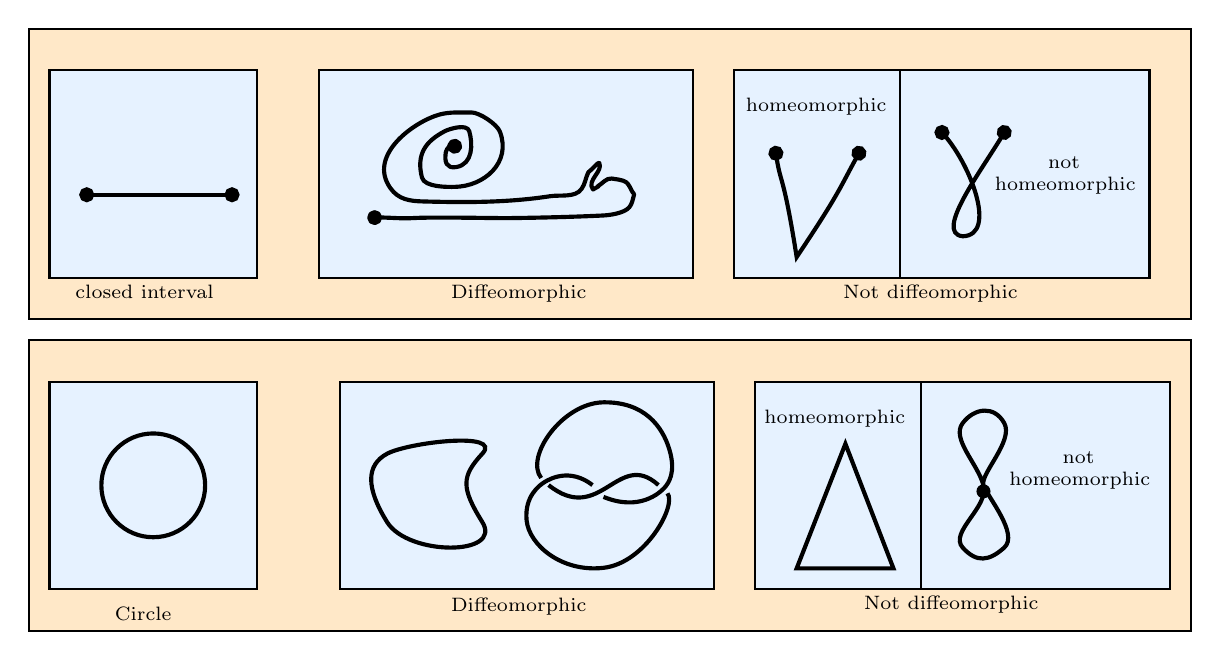
\begin{tikzpicture}[x=0.75pt,y=0.75pt,yscale=-1,xscale=1]
		%uncomment if require: \path (0,300); %set diagram left start at 0, and has height of 300
		
		%Shape: Rectangle [id:dp5759997839543596] 
		\draw  [fill={rgb, 255:red, 255; green, 232; blue, 200 }  ,fill opacity=1 ] (40,157) -- (600,157) -- (600,297) -- (40,297) -- cycle ;
		%Shape: Rectangle [id:dp09502642053448573] 
		\draw  [fill={rgb, 255:red, 255; green, 232; blue, 200 }  ,fill opacity=1 ] (40,7) -- (600,7) -- (600,147) -- (40,147) -- cycle ;
		%Shape: Rectangle [id:dp794045496594401] 
		\draw  [fill={rgb, 255:red, 230; green, 242; blue, 255 }  ,fill opacity=1 ] (50,27) -- (150,27) -- (150,127) -- (50,127) -- cycle ;
		%Straight Lines [id:da6087895159341825] 
		\draw [line width=1.5]    (67.96,87) -- (110,87) -- (137.96,87) ;
		\draw [shift={(137.96,87)}, rotate = 0] [color={rgb, 255:red, 0; green, 0; blue, 0 }  ][fill={rgb, 255:red, 0; green, 0; blue, 0 }  ][line width=1.5]      (0, 0) circle [x radius= 2.61, y radius= 2.61]   ;
		\draw [shift={(67.96,87)}, rotate = 0] [color={rgb, 255:red, 0; green, 0; blue, 0 }  ][fill={rgb, 255:red, 0; green, 0; blue, 0 }  ][line width=1.5]      (0, 0) circle [x radius= 2.61, y radius= 2.61]   ;
		%Shape: Rectangle [id:dp09862432189325276] 
		\draw  [fill={rgb, 255:red, 230; green, 242; blue, 255 }  ,fill opacity=1 ] (180,27) -- (360,27) -- (360,127) -- (180,127) -- cycle ;
		%Curve Lines [id:da7044859223189306] 
		\draw [line width=1.5] [line join = round][line cap = round]   (206.67,98) .. controls (212.79,97.77) and (218.84,98.62) .. (224.95,98.25) .. controls (235.26,97.63) and (264.87,98.34) .. (271.54,98.25) .. controls (286.57,98.05) and (301.61,97.71) .. (316.62,97) .. controls (319.63,96.86) and (326.92,95.98) .. (329.4,92.99) .. controls (330.76,91.34) and (331.06,89.03) .. (331.65,86.97) .. controls (331.78,86.5) and (331.16,86.13) .. (330.9,85.71) .. controls (330.36,84.84) and (329.2,81.93) .. (327.89,80.95) .. controls (326.37,79.8) and (322.33,79.43) .. (320.88,79.19) .. controls (318.33,78.78) and (316.36,81.67) .. (314.12,82.95) .. controls (313.62,83.24) and (316.75,81.75) .. (311.86,84.46) .. controls (308.57,80.06) and (317.01,75.65) .. (314.87,71.67) .. controls (314.51,71.01) and (311.61,74.68) .. (309.61,76.18) .. controls (308.2,79.09) and (308.2,81.56) .. (306.35,84.21) .. controls (303.36,88.5) and (296.24,86.93) .. (291.08,87.72) .. controls (270.68,90.82) and (251.05,90.76) .. (230.21,90.23) .. controls (223.63,90.06) and (218.16,89.37) .. (214.18,83.71) .. controls (203.05,67.86) and (225.81,51.67) .. (237.98,48.34) .. controls (242.9,47) and (248.15,47.41) .. (253.26,47.34) .. controls (257.1,47.29) and (265.65,52.98) .. (267.03,56.62) .. controls (272.72,71.56) and (259.41,82.95) .. (245.24,83.21) .. controls (242.23,83.26) and (230.67,83.51) .. (229.46,78.69) .. controls (226.65,67.44) and (231.14,61.28) .. (240.48,56.37) .. controls (242.38,55.37) and (251.15,52.51) .. (252.25,56.37) .. controls (254,62.5) and (254.12,72.26) .. (245.99,73.67) .. controls (241.17,74.51) and (240.2,71.1) .. (240.98,66.4) .. controls (241.21,65.02) and (243.76,61.42) .. (245.24,63.64) ;
		\draw [shift={(245.24,63.64)}, rotate = 56.35] [color={rgb, 255:red, 0; green, 0; blue, 0 }  ][fill={rgb, 255:red, 0; green, 0; blue, 0 }  ][line width=1.5] [line join = round][line cap = round]     (0, 0) circle [x radius= 2.61, y radius= 2.61]   ;
		\draw [shift={(206.67,98)}, rotate = 357.79] [color={rgb, 255:red, 0; green, 0; blue, 0 }  ][fill={rgb, 255:red, 0; green, 0; blue, 0 }  ][line width=1.5] [line join = round][line cap = round]     (0, 0) circle [x radius= 2.61, y radius= 2.61]   ;
		%Shape: Rectangle [id:dp17014344801268177] 
		\draw  [fill={rgb, 255:red, 230; green, 242; blue, 255 }  ,fill opacity=1 ] (460,27) -- (580,27) -- (580,127) -- (460,127) -- cycle ;
		%Shape: Rectangle [id:dp22662056681483733] 
		\draw  [fill={rgb, 255:red, 230; green, 242; blue, 255 }  ,fill opacity=1 ] (380,27) -- (460,27) -- (460,127) -- (380,127) -- cycle ;
		%Curve Lines [id:da6145254850720514] 
		\draw [line width=1.5]    (510,57) .. controls (499.75,74.5) and (475.75,105.5) .. (490,107) .. controls (507.25,106.5) and (493.25,71) .. (480,57) ;
		\draw [shift={(480,57)}, rotate = 226.58] [color={rgb, 255:red, 0; green, 0; blue, 0 }  ][fill={rgb, 255:red, 0; green, 0; blue, 0 }  ][line width=1.5]      (0, 0) circle [x radius= 2.61, y radius= 2.61]   ;
		\draw [shift={(510,57)}, rotate = 120.36] [color={rgb, 255:red, 0; green, 0; blue, 0 }  ][fill={rgb, 255:red, 0; green, 0; blue, 0 }  ][line width=1.5]      (0, 0) circle [x radius= 2.61, y radius= 2.61]   ;
		%Shape: Rectangle [id:dp31913409751177024] 
		\draw  [fill={rgb, 255:red, 230; green, 242; blue, 255 }  ,fill opacity=1 ] (50,177) -- (150,177) -- (150,277) -- (50,277) -- cycle ;
		%Shape: Rectangle [id:dp035182155141359805] 
		\draw  [fill={rgb, 255:red, 230; green, 242; blue, 255 }  ,fill opacity=1 ] (190,177) -- (370,177) -- (370,277) -- (190,277) -- cycle ;
		%Shape: Rectangle [id:dp7290551523037767] 
		\draw  [fill={rgb, 255:red, 230; green, 242; blue, 255 }  ,fill opacity=1 ] (470,177) -- (590,177) -- (590,277) -- (470,277) -- cycle ;
		%Shape: Rectangle [id:dp9828205444947584] 
		\draw  [fill={rgb, 255:red, 230; green, 242; blue, 255 }  ,fill opacity=1 ] (390,177) -- (470,177) -- (470,277) -- (390,277) -- cycle ;
		%Shape: Circle [id:dp8999286469461747] 
		\draw  [line width=1.5]  (75,227) .. controls (75,213.19) and (86.19,202) .. (100,202) .. controls (113.81,202) and (125,213.19) .. (125,227) .. controls (125,240.81) and (113.81,252) .. (100,252) .. controls (86.19,252) and (75,240.81) .. (75,227) -- cycle ;
		%Shape: Regular Polygon [id:dp619536170202954] 
		\draw  [line width=1.5]  (212.65,211.78) .. controls (222.84,206.3) and (268.73,200.82) .. (258.53,211.78) .. controls (248.34,222.74) and (248.34,228.22) .. (258.53,244.67) .. controls (268.73,261.11) and (222.84,261.11) .. (212.65,244.67) .. controls (202.45,228.22) and (202.45,217.26) .. (212.65,211.78) -- cycle ;
		%Curve Lines [id:da7142664625345396] 
		\draw [line width=1.5]    (290.47,226.87) .. controls (315.47,246.81) and (323.94,209.21) .. (343.39,226.87) ;
		%Curve Lines [id:da5535164021641068] 
		\draw [line width=1.5]    (286.9,223.45) .. controls (278.85,213.26) and (297.22,187.28) .. (316.93,187) .. controls (336.64,186.71) and (345.37,198.67) .. (348.68,209.78) .. controls (351.99,220.89) and (348.28,226.02) .. (346.17,228.29) .. controls (344.05,230.57) and (334.26,239.69) .. (316.93,232.57) ;
		%Curve Lines [id:da772702812520371] 
		\draw [line width=1.5]    (347.76,230.86) .. controls (352.28,236.59) and (337.17,264.47) .. (316.93,266.74) .. controls (296.69,269.02) and (281.08,255.64) .. (279.89,243.96) .. controls (278.7,232.28) and (286.14,226.88) .. (288.49,225.45) .. controls (290.83,224.01) and (300.57,218.32) .. (311.64,226.87) ;
		
		%Shape: Triangle [id:dp7950611477426] 
		\draw  [line width=1.5]  (433.48,207) -- (456.62,267) -- (410,267) -- cycle ;
		%Shape: Polygon Curved [id:ds6158924144504883] 
		\draw  [line width=1.5]  (490,197) .. controls (495.75,189.5) and (505.25,188.5) .. (510,197) .. controls (514.75,205.5) and (498.18,221.64) .. (500,227) .. controls (501.82,232.36) and (517.25,250.5) .. (510,257) .. controls (502.75,263.5) and (496.75,264.5) .. (490,257) .. controls (483.25,249.5) and (502.75,237.5) .. (500,227) .. controls (497.25,216.5) and (484.25,204.5) .. (490,197) -- cycle ;
		%Shape: Circle [id:dp2069132244539451] 
		\draw  [fill={rgb, 255:red, 0; green, 0; blue, 0 }  ,fill opacity=1 ] (497.13,229.88) .. controls (497.13,228.29) and (498.41,227) .. (500,227) .. controls (501.59,227) and (502.88,228.29) .. (502.88,229.88) .. controls (502.88,231.46) and (501.59,232.75) .. (500,232.75) .. controls (498.41,232.75) and (497.13,231.46) .. (497.13,229.88) -- cycle ;
		%Curve Lines [id:da9430641490320497] 
		\draw [line width=1.5]    (400,67) .. controls (402.25,83) and (403.25,74.5) .. (410,117) .. controls (431.75,84.5) and (430.75,83.5) .. (440,67) ;
		\draw [shift={(440,67)}, rotate = 299.28] [color={rgb, 255:red, 0; green, 0; blue, 0 }  ][fill={rgb, 255:red, 0; green, 0; blue, 0 }  ][line width=1.5]      (0, 0) circle [x radius= 2.61, y radius= 2.61]   ;
		\draw [shift={(400,67)}, rotate = 82] [color={rgb, 255:red, 0; green, 0; blue, 0 }  ][fill={rgb, 255:red, 0; green, 0; blue, 0 }  ][line width=1.5]      (0, 0) circle [x radius= 2.61, y radius= 2.61]   ;
		
		% Text Node
		\draw (61,129) node [anchor=north west][inner sep=0.75pt]  [font=\scriptsize] [align=left] {closed interval};
		% Text Node
		\draw (80,284) node [anchor=north west][inner sep=0.75pt]  [font=\scriptsize] [align=left] {Circle};
		% Text Node
		\draw (242,129) node [anchor=north west][inner sep=0.75pt]  [font=\scriptsize] [align=left] {Diffeomorphic};
		% Text Node
		\draw (431,129) node [anchor=north west][inner sep=0.75pt]  [font=\scriptsize] [align=left] {Not diffeomorphic};
		% Text Node
		\draw (384,39) node [anchor=north west][inner sep=0.75pt]  [font=\scriptsize] [align=left] {homeomorphic};
		% Text Node
		\draw (504,67) node [anchor=north west][inner sep=0.75pt]  [font=\scriptsize] [align=left] {\begin{minipage}[lt]{49.95pt}\setlength\topsep{0pt}
				\begin{center}
					not\\homeomorphic
				\end{center}
				
		\end{minipage}};
		% Text Node
		\draw (242,280) node [anchor=north west][inner sep=0.75pt]  [font=\scriptsize] [align=left] {Diffeomorphic};
		% Text Node
		\draw (441,279) node [anchor=north west][inner sep=0.75pt]  [font=\scriptsize] [align=left] {Not diffeomorphic};
		% Text Node
		\draw (511,209) node [anchor=north west][inner sep=0.75pt]  [font=\scriptsize] [align=left] {\begin{minipage}[lt]{49.95pt}\setlength\topsep{0pt}
				\begin{center}
					not\\homeomorphic
				\end{center}
				
		\end{minipage}};
		% Text Node
		\draw (393,189) node [anchor=north west][inner sep=0.75pt]  [font=\scriptsize] [align=left] {homeomorphic};
		
		
	\end{tikzpicture}
\end{figure}
	
According to the two following propositions, in a \emph{smooth} manifold, the coordinate maps are diffeomorphisms, and conversely, any diffeomorphism from an open subset of the manifold to an open subset of a Euclidean space can serve as a coordinate map. 

\begin{proposition}[Coordinate maps are diffeomorphisms]
	If $ (U,\phi) $ is a chart on a manifold $ M $ of dimension $ n $, then the coordinate map $ \phi:U\to\phi(\phi) \in \R^n$ is a diffeomorphism.
\end{proposition}
\begin{proof}
	For the proof, we will use the notion of smooth maps between manifolds in a smart way! First, observe that since $ \phi $ is a coordinate map, thus it is automatically a homeomorphism. Thus we just need to show that $ \phi $ and $ \inv{\phi} $ are smooth. Let $ U $ be a manifold with an atlas $ \set{(U,\phi)} $. Also, let $ \phi(U) \subset\R^n $ be a manifold (this is indeed a manifold as it is an open subset of a Euclidean space), with an atlas $ \set{(\phi(U),\mathds{1}_{\phi(U)})} $. In this point of view, the coordinate map $ \phi $ is in fact a map between manifolds. This is smooth, since 
	\[ \mathds{1}_{\phi(U)}\circ \phi\circ \inv{\phi}: \underbrace{\phi(U \cap \inv{\phi}(\phi(U)))}_{\phi(U)} \to \phi(U) \]
	is smooth, then by \autoref{prop:smoothnessInTermsOfCharts} $ (ii) \implies (i) $, the map $ \phi $ is smooth.
	
	To show the smoothness of the map $ \inv{\phi} $, we observe that this is a map from the manifold with atlas $ \set{(\phi(U),\inv{\phi})} $ to the manifold with atlas $ \set{(U,\phi)} $. Since the following map
	\[ \phi \circ \inv{\phi} \circ \mathds{1}_{\phi(U)}: \phi(U) \to \phi(U) \]
	is smooth (since it is just the identity map), then by \autoref{prop:smoothnessInTermsOfCharts} $ (ii) \implies (i) $ the map $ \inv{\phi} $ is smooth.
	
	Putting these two results together, we have shown that the coordinate map $ \phi $ is indeed a diffeomorphism from $ U $ to $ \R^n $.
\end{proof}


The following proposition is the converse of the proposition above.

\begin{proposition}
	Let $ U $ be an open subset of a manifold $ M $ of dimension $ n $. If $ F: U \to F(U) \subset \R^n $ is a diffeomorphism onto an open subset of $ \R^n $, then $ (F,U) $ is a chart in the differentiable structure of $ M $.
\end{proposition}
\begin{proof}
	Since $ F $ is a diffeomorphism, then it is certainly a homeomorphism. 
	Thus we just need to show that $ (U,F) $ is a chart, i.e. compatible with the maximal atlas of the manifold (note that since $ M $ is an smooth manifold, then there exists a maximal atlas). Let $ p \in  U $ and let $ (V,\psi) $ be a chart that contains $ p $. Then consider the function
	\[ F \circ \inv{\psi}: \psi(U\cap V) \to F(U\cap V) \qquad \psi\circ \inv{F}: F(U\cap V) \to \psi(U\cap V). \]
	By the proposition above, we know that since $ \phi $ is a coordinate chart of a smooth manifold, then $ \phi $ and $ \inv{\phi} $ are both smooth. Then the functions above are a composition of smooth functions, thus they are smooth as well. This proves that $ (U,F) $ is compatible with the chart $ (V,\psi) $. Since this chart was arbitrary, then it is compatible with the whole atlas, thus $ (U,F) $ is a chart. Also, by the maximality of the atlas, $  (U,F) $ is contained in the atlas.
\end{proof}

Now using the notion of smooth maps between manifolds, we can define a Lie group.
\begin{definition}[Lie group]
	A \emph{Lie group} is a $ C^\infty $ manifold $ G $ having a group structure such that the multiplication map
	\[ \mu: G\times G \to G \]
	and the inverse map
	\[ \iota: G\to G, \qquad \iota(x) = \inv{x}, \]
	are both $ C^\infty $.
\end{definition}

\begin{remark}
	Similar to the definition above, a topological group is a topological space having a group structure such that the multiplication and the inverse maps are both continuous. Note that a topological group is required to be a topological space, but not a topological manifold.
\end{remark}

The followings are some examples of Lie groups. We can easily check the group operation and the inverse map are both smooth by using the definitions that we have had above.

\begin{enumerate}[(i)]
	\item The Euclidean space $ \R^n $ is a Lie group under addition.
	\item The set $ \C^{\times} $ of nonzero complex numbers is a Lie group under multiplications.
	\item Subsequently, the unit circle in $ \C^\times $ is a Lie group under multiplication.
\end{enumerate}


\section{Partial Derivatives}
In this section we will define the notion of partial derivatives of the maps between manifolds. We will use the notion of coordinate charts for this definition. Let $ N $ be a manifold of dimension $ n $, and let $ (r^1,\cdots,r^n) $ be the standard coordinate function on $ \R^n $. For a chart $ (U,\phi) $ on the manifold, $ \phi $ is a vector valued function on manifold. We denote its coordinate functions as $ x^i $ where $ x^i = r^i \circ \phi $. This is just a fancy (but very useful) way of writing the $ i\text{-th}$ coordinate of the vector valued function $ \phi $. Now we can define the directional derivatives for the functions on manifolds.

\begin{definition}[Directional derivative]
	Let $ N $ be a manifold, and $ f:N \to \R $ an smooth function. Let $ p\in U $ and $ (U,\phi) $ any chart containing $ p $, where $ \phi = (x^1,\cdots,x^n) $. We define the direction derivative of $ f $ at $ p $ as 
	\[ \frac{\partial f}{\partial x^i}(p) = \frac{\partial (f\circ \inv{\phi})}{\partial r^i}(\phi(p)) = \frac{\partial}{\partial r^i}\big|_{\phi(p)} (f\circ\inv{\phi}). \]
\end{definition}

\begin{remark}
	In the definition above, we can re-write it as
	\[ \frac{\partial f}{\partial x^i}(p) =\frac{\partial f}{\partial x^i}(\underbrace{\inv{\phi}(\phi(p))}_{p}) = \frac{\partial (f\circ \inv{\phi})}{\partial r^i}(\phi(p)). \]
	We can now write
	\[ \frac{\partial (f\circ \inv{\phi})}{\partial r^i} =\frac{\partial f}{\partial x^i} \circ \inv{\phi} = [\inv{\phi}]^* [\frac{\partial f}{\partial x^i}],  \]
	where shows that $ \frac{\partial (f\circ \inv{\phi})}{\partial r^i} $ is the pull back of the function $ \frac{\partial f}{\partial x^i} $ when viewed as a function on the manifold. Since the pull back of $ \frac{\partial f}{\partial x^i} $ is smooth (as $ f\circ \inv{\phi} $ is smooth), then $ \frac{\partial f}{\partial x^i} $ is smooth when viewed as a real valued function on the manifold.
\end{remark}

\begin{proposition}
	Suppose $ (U,x^1,\cdots,x^n) $ is a chart on a manifold. Then we have
	\[ \frac{\partial x^i}{\partial x^j} = \delta^i_j. \]
\end{proposition}
\begin{proof}
	We view $ x^i $ as a real valued function on the manifold. For a point $ p $ in the manifold, we can use the definition of partial derivative to write
	\[ \frac{\partial x^i}{\partial x^j}(p) = \frac{\partial (x^i \circ \inv{\phi})}{\partial r^j} = \frac{\partial (r^i \circ \phi \circ \inv{\phi})}{\partial r^j} = \frac{\partial r^i}{\partial r^j} = \delta^i_j. \]
	Note that we have used the fact that $ \phi = (x^1,\cdots,x^n) $.
\end{proof}

Using the notion of partial derivatives, we can define the notion of Jacobian matrix for the maps between manifolds.

\begin{definition}[Jacobian matrix of maps between manifolds]
	Let $ F:N \to M $ be a smooth map, and let $ (U,\phi) = (U,x^1,\cdots,x^n) $ and $ (V,\psi) = (V,y^1,\cdots,y^m) $ be charts on $ N $ and $ M $ respectively such that $ F(U) \subset V $. Denote by
	\[ F^i = y^i \circ F = r^i \circ \psi \circ F : U \to \R \]
	the $ i\text{-th} $ component of $ F $ in the chart $ (V,\psi) $. The following matrix
	\[ J = \left[ \frac{\partial F^i}{\partial x^j} \right] \]
	is called the Jacobian matrix of $ F $ relative to the charts given as above. In case $ M,N $ have the same dimension, the determinant of this matrix is called the Jacobian determinant of $ F $ relative to the two charts. The Jacobian determinant is also written as 
	\[ \det(J) = \frac{\partial (F^1,\cdots,F^n)}{\partial(x^1,\cdots,x^n)}. \]
\end{definition}

\section{Inverse function theorem}
As we studied before, on a manifold $ N $ of dimension $ n $, a diffeomorphism $ f: U \to \R^n $ is indeed a coordinate map. In this section, we want to study the conditions under which a smooth map between manifolds can be upgraded to a local diffeomorphism. For this end, we will use a slight generalization of the inverse function theorem in the Euclidean spaces.

\begin{definition}[Inverse function theorem in Euclidean spaces]
	Let $ F: W \to \R^n $ where $ W \subset \R^n $ be a smooth map. We say this function is a \emph{local diffeomorphism} or locally invertible at point $ p $, if there exists an open set $ U \subset W $ containing $ p $ such that the Jacobian determinant is non-zero at $ p $, i.e.
	\[ \det \left[  \frac{\partial F^i}{\partial r^j} \right](p) \neq 0.  \]
\end{definition}
We will skip proving this theorem here and we will just use it to prove the generalized version of this theorem for smooth maps between manifolds.

\begin{definition}[Inverse function theorem for manifolds]
	Let $ F: N \to M $ be a smooth map between two manifolds of the same dimension, and $ p \in N $. Suppose for some charts $ (U,\phi) = (U,x^1,\cdots,x^n) $ about $ p $ in $ N $ and $ (V,\psi) = (V,y^1,\cdots,y^n)$ about $ F(p) $ in $ M, F(U) \subset V $. Set $ F^i = y^i \circ F $. Then $ F $ is locally invertible at $ p $ if and only if its Jacobian determinant $ \det(\partial F^i/\partial x^j)(p) $ is nonzero.
\end{definition}
\begin{proof}
	First, observe the proof structure in the observation box below. We just need to show two following bi-directional implications.
	\[ F \text{ is locally invertible} \Longleftrightarrow \psi\circ F \circ \inv{\phi} \text{ is locally invertible.} \]
	and also
	\[ \det \left[ \frac{\partial (\psi\circ F \circ \inv{\phi})^i}{\partial r^j}  \right](\phi(p)) \neq 0 \Longleftrightarrow \det\left[ \frac{\partial F^i}{\partial x^j} \right](p) \neq 0. \]
	
	For the first bi-directional implication since $ \phi,\psi $ are coordinate maps, thus are invertible (they are bijective) and from the composition of functions it follows that the bi-directional implication is true.
	
	For the second bi-directional implication we start with the forward direction. We can write
	\[ \frac{\partial (\psi\circ F \circ \inv{\phi})^i}{\partial r^j} = \frac{\partial (r^i \circ \psi \circ F \circ \inv{\phi})}{\partial r^j} = \frac{\partial(y^i\circ F\circ \inv{\phi})}{\partial r^j} = \frac{\partial( F^i \circ \inv{\phi})}{\partial r^j} =  \frac{\partial F^i}{\partial x^j}. \]
	This proves the forward direction. We can do this starting from the last equation which proves the backward direction.
\end{proof}

\begin{observation}[Some hidden treasures!]
	When proving the theorem above, we can figure out what should be the structure of the proof, even if we can not demonstrate the proof steps completely. For me, there is some sense of dimensional analysis if physics in what I am saying. By looking only at the ingredients of the problem/theorem/etc, we can figure out what is the possible way that we can combine those ingredients to achieve to a full proof. The following figure reveals this structure for the proof.
\end{observation}
	\begin{figure}[h!]
	\centering
	
	
	
	\tikzset{every picture/.style={line width=0.75pt}} %set default line width to 0.75pt        
	
	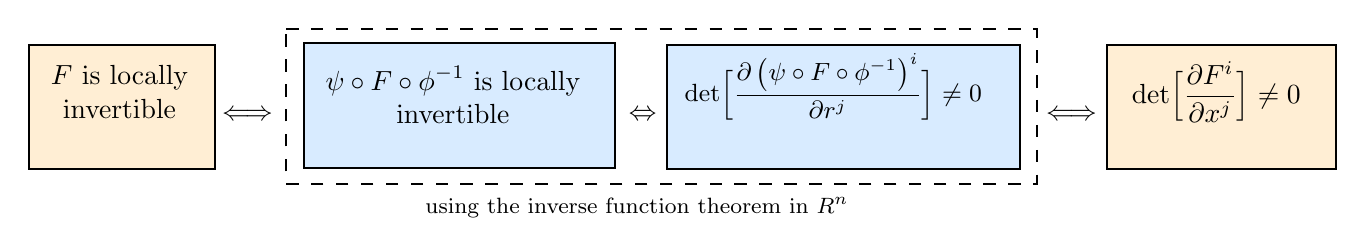
\begin{tikzpicture}[x=0.75pt,y=0.75pt,yscale=-1,xscale=1]
		%uncomment if require: \path (0,300); %set diagram left start at 0, and has height of 300
		
		%Shape: Rectangle [id:dp28925530323831317] 
		\draw  [fill={rgb, 255:red, 154; green, 203; blue, 255 }  ,fill opacity=0.39 ] (143,39.33) -- (292.67,39.33) -- (292.67,99.33) -- (143,99.33) -- cycle ;
		%Shape: Rectangle [id:dp34966788396180615] 
		\draw  [fill={rgb, 255:red, 154; green, 203; blue, 255 }  ,fill opacity=0.39 ] (318,40) -- (488,40) -- (488,100) -- (318,100) -- cycle ;
		%Shape: Rectangle [id:dp8415325367676847] 
		\draw  [fill={rgb, 255:red, 255; green, 203; blue, 120 }  ,fill opacity=0.32 ] (10.33,40) -- (100,40) -- (100,100) -- (10.33,100) -- cycle ;
		%Shape: Rectangle [id:dp9745265751684289] 
		\draw  [fill={rgb, 255:red, 255; green, 203; blue, 120 }  ,fill opacity=0.32 ] (530,40) -- (640,40) -- (640,100) -- (530,100) -- cycle ;
		%Shape: Rectangle [id:dp35176055981313437] 
		\draw  [dash pattern={on 4.5pt off 4.5pt}] (134.33,32.33) -- (496,32.33) -- (496,107) -- (134.33,107) -- cycle ;
		
		% Text Node
		\draw (17,48.67) node [anchor=north west][inner sep=0.75pt]   [align=left] {\begin{minipage}[lt]{53.36pt}\setlength\topsep{0pt}
				\begin{center}
					$\displaystyle F$ is locally \\invertible
				\end{center}
				
		\end{minipage}};
		% Text Node
		\draw (148,49) node [anchor=north west][inner sep=0.75pt]   [align=left] {\begin{minipage}[lt]{97.77pt}\setlength\topsep{0pt}
				\begin{center}
					$\displaystyle \psi \circ F\circ \phi ^{-1}$ is locally \\invertible
				\end{center}
				
		\end{minipage}};
		% Text Node
		\draw (319,43) node [anchor=north west][inner sep=0.75pt]  [font=\small] [align=left] {\begin{minipage}[lt]{116.2pt}\setlength\topsep{0pt}
				\begin{center}
					$\displaystyle \det\Bigl[\frac{\partial \left( \psi \circ F\circ \phi ^{-1}\right)^{i}}{\partial r^{j}}\Bigr] \neq 0$ 
				\end{center}
				
		\end{minipage}};
		% Text Node
		\draw (531.67,46.67) node [anchor=north west][inner sep=0.75pt]   [align=left] {\begin{minipage}[lt]{74pt}\setlength\topsep{0pt}
				\begin{center}
					$\displaystyle \det\Bigl[\frac{\partial F^{i}}{\partial x^{j}}\Bigr] \neq 0$ 
				\end{center}
				
		\end{minipage}};
		% Text Node
		\draw (298,70) node [anchor=north west][inner sep=0.75pt]    {$\Leftrightarrow $};
		% Text Node
		\draw (200,112) node [anchor=north west][inner sep=0.75pt]  [font=\footnotesize] [align=left] {using the inverse function theorem in $\displaystyle \mathbb{R}^{n}$};
		% Text Node
		\draw (102,70) node [anchor=north west][inner sep=0.75pt]    {$\Longleftrightarrow $};
		% Text Node
		\draw (499,70) node [anchor=north west][inner sep=0.75pt]    {$\Longleftrightarrow $};
		
		
	\end{tikzpicture}
\end{figure}
	
\begin{corollary}
	Let $ N $ be a manifold of dimension $ n $. A set of $ n $ smooth functions $ F^1,\dots,F^n $ defined on a coordinate neighborhood $ (U,x^1,\cdots,x^n) $ of a point $ p \in N $ forms a coordinate system about $ p $ if and only if the Jacobian determinant 
	\[ \left[  \frac{\partial F^i}{\partial x^j}  \right](p) \neq 0. \]
\end{corollary}

\section{Summary}
\begin{summary}[A useful thing!]
	Let $ N $ be a manifold of dimension $ n $, and $ (U,\phi) $ a local coordinate system containing $ p \in N $. Then $ \phi $ can be viewed as a vector valued real function $ \phi:U \to \R^n $. Let $ r^i $ be the standard coordinate functions of $ \R^n $. Then the $ i\text{-th} $ of $ \phi $ can be written as.
	\[ x^i = r^i \circ \phi . \]
\end{summary}

\begin{proof}
	define the vector valued function as $ F = (F^1,\cdots,F^n) $. Then we have
	\begin{itemize}
		\item[$\,$] $ \det[\partial F^i/\partial x^j] \neq 0 $.
		\item[$\Longleftrightarrow$] $ F $ is locally invertible.
		\item[$\Longleftrightarrow$] There is a neighborhood $ W $ containing $ p $ such that $ F:W \to F(W) \subset \R^n $ is a diffeomorphism.
		\item[$\Longleftrightarrow$] $ (W,F) $ is a coordinate system in the maximal atlas of $ N $.
	\end{itemize}
\end{proof}




\section{Quotients}
The quotient construction is a process of simplification. Starting with an equivalence relation on a set, we identify each equivalence class to a point. If the original set is a topological space, then it is always possible to give the quotient space a topology so that the natural projection map (i.e. $ \pi: S\to S/\sim\ ,\ x\mapsto [x] $) becomes continuous. However, if the original set is a manifold, then it is not always true that the quotient set is also manifold, as the conditions like being Hausdorff or second countable might break.

\begin{definition}[Quotient topology]
	Let $ (X,\mathcal{T}) $ be a topological space, and $ \sim $ an equivalence relation with $ \pi $ as the natural projection map. A set $ U \in X/\sim $ is open, if and only if $ \inv{\pi}(U) \in \mathcal{T} $, i.e. open. 
\end{definition}
\begin{remark}
	In the definition above, clearly the empty set $ \emptyset $ and the whole quotient space $ X/\sim $ are open. That is because $ \inv{\pi}(\emptyset) = \emptyset \in \mathcal{T} $ (since the equivalence relation $ \sim $ partitions the set), and $ \inv{\pi}(X/\sim) = X \in \mathcal{T}  $. Also, for any map, in particular $ \pi $ we have
	\[ \inv{\pi}(\bigcup_\alpha U_\alpha) = \bigcup_\alpha \inv{\pi}(U_\alpha), \qquad \inv{\pi}(\bigcap_i U_i) = \bigcap_i \inv{\pi}(U_i) \]
	where $ \inv{\pi}(U) $ means the pre-image of the set $ U $ under the map $ \phi $. This shows that an arbitrary union of the open sets in the quotient space is open, and also a finite intersection of open sets of the quotient space is also open. Thus the space $ (X/\sim, \mathcal{T}') $ where $ U \in \mathcal{T}' $ if and only if $ \inv{\pi}(U) \in \mathcal{T} $ is a topological space.
	\newline 
	\noindent Also Note that since $ \inv{\pi} $ maps open sets of $ X/\!\sim $ to the open sets of $ X $, then $ \pi $ is automatically (i.e. by design) a continuous function.
\end{remark}

\subsection{Continuity of a map on a Quotient}

Let $ S $ be a topological space and $ \sim $ and equivalence relation on this set. Give the quotient set $ S/\sim $ the quotient topology. Then a function $ f:S\to Y $ from $ S $ to another topological space, where it is constant for all elements in the same equivalence class. This map then induces a map on $ S/\sim $, i.e. $ \bar{f}: S/\sim \to Y $ where
 \[ \bar{f}([p]) = f(p) \qquad \text{for $ p\in S $}. \] 
 or in other words
 \[ \bar{f}(\pi(p)) = f(p) \qquad \text{or equivalently} \qquad \bar{f}\circ\pi  = f. \]

\begin{proposition}
	\label{prop:ContinousInducedmap}
	The induced map $ \bar{f}:S/\sim \to Y $ is continuous if and only if the map $ f: S \to Y $ is continuous.
\end{proposition}
\begin{solution}
	First, we will show that continuity of $ \bar{f} $ implies the continuoity of $ f $. Let $ U \in \mathcal{T}_Y $. Since $ \bar{f} $ is continuous, then $ \inv{\bar{f}}(U) \in \mathcal{T}_{S/\sim} $. Furthermore, since $ \pi $ is continuous then $ \inv{\pi}(\inv{\bar{f}}(U)) \in \mathcal{T}_{S} $, thus $ (\bar{f}\circ \pi) $ is continuous. Since $  f = \bar{f}\circ \pi $, then $ f $ is also continuous. As an alternative prove, we could start with the fact that $ f = \bar{f}\circ \pi $, and since $ \bar{f} $ and $ \pi $ are both continuous, then so is $ f $.
	
	For the converse, we want to show that the continuoity of $ f $ implies the continuoity of $ \inv{f} $. Let $ V \in \mathcal{T}_Y $. Since $ f $ is continuous, then $ \inv{f}(V) \in \mathcal{T}_S $. On the other hand, we have $ \inv{f}(V) =( \inv{\pi}\circ \inv{\bar{f}})(V) $. Since $ \inv{\pi} $ sends open sets to open sets, then $ \bar{f}(V) \in \mathcal{T}_{S/\sim} $. Thus $ \bar{f} $ is continuous.
\end{solution}

\begin{definition}[Identification of a subset to a point]
	Let $ S $ be a topological space and $ A \subset S $. Let $ \sim $ be s relation on $ S $ where 
	\[ x\sim x \qquad \forall x \in S, \]
	and also
	\[ x\sim y \qquad \forall x,y \in A. \]
	This is an equivalence relation on $ S $. We call the quotient space $ S/\sim $ is obtained from $ S $ by identifying the set $ A $ to a point.
\end{definition}

\section{A Necessary Condition for a Hausdorff Space}
The quotient construction often does not preserve the second countablity and Hausdorff property of a topological space. We start with the following proposition.

\begin{proposition}
	Let $ X $ be a topological space, and $ \sim $ an equivalence relation on $ X $. If $ X/\sim $ is Hausdorff then equivalent class $ [p] $ of any $ p \in X $ is closed in $ X $.
\end{proposition}
\begin{proof}
	In a Hausdorff space, every singleton set is closed. let $ p \in X $. Then $ \set{\pi(p)} $ is closed in $ X/\sim $. Since $ \pi $ is continuous, then the pre image $ \inv{\pi}(\set{\pi(p)}) = [p] $ is closed in $ X $. This completes the proof.
\end{proof}

\begin{remark}
	In the proof above, we claimed that in a Hausdorff space, every singleton set is closed. To see this, let $ p \in S $ a Hausdorff space. Consider the singleton $ \set{p} $ and its complement, i.e. $ S - \set{p} $. We claim that set $ S - \set{p} $ is open. To show this, let $ U \in \mathcal{T} $ where $ p \in U $. Since $ S $ is Hausdorff, then there exists an open set $ V \in \mathcal{T} $ such that contains any point $ q \in S - \set{p} $ and do not overlap with $ U $. This $ q \in V \subset S - \set{p} $. Thus for every point $ S - \set{p} $ we can find an open set containing $ q $ that is contained in the set $ S - \set{p} $.
\end{remark}

\begin{definition}[Open equivalence relation]
	Let $ \sim $ be an equivalence relation defined on a set. This equivalence relation is said to be open, if $ \pi(U) $ is open for some open set $ U $
\end{definition}
\begin{remark}
	\label{remark:OpenEquivReleation}
	We can give a useful characterization of open equivalence relations. Let $ U $ be an open set. Then $ \pi(U) $ being open means that $ \inv{\pi}(\pi(U)) $ is also open. Thus an equivalence relation is open if and only if 
	\[ \inv{\pi}(\pi(U)) = \bigcup_{x \in  U} [x] \]
	is open.
\end{remark}

\begin{theorem}
	\label{thm:QuotientIsHausdorff}
	Let $ S $ be a topological space, and $ \sim $ an open equivalence relation defined on $ S $. Then $ S/\sim $ is Hausdorff if and only if the graph $ R $ of the relation is closed in $ S\times S $.
\end{theorem}
\begin{proof}
	First, consider the following chain of bidirectional implications.
	
	\begin{itemize}[noitemsep]
		\item [] $ R $ is closed in $ S\times S $
		\item [$ \biImp $] $ S\times S - R $ is closed in $ S\times S $
		\item [$ \biImp $] For all $ (x,y) \in (S\times S) - R $, there exist an open cell $ U\times V \ni (x,y) $ such that $ U\times V \cap R = \emptyset $.
		\item [$ \biImp $] For all pair $ x,y \in S $ where $ x\not\sim y $, there exists open sets $ U\ni x $ and $ V \ni y $ such that no element of $ U $ is equivalent to an element of $ V $. 
		\item [$ \biImp $] For all two points in $ [x]\neq [y] \in S/\sim $ there exists open sets $ U\ni x,V \ni y $ open in $ S $ such that $ \pi(U) \cap \pi(V)  = \emptyset $. 
	\end{itemize}
		Now what remains to show is to show that the last statement (call it statement *) is equivalent to being Hausdorff. If $ * $ is true, then since $ \pi $ is open, then $ S/\sim $ being Hausdorff follows immediately. For the converse, if $ S/\sim $ Hausdorff, then for $ [x]\neq [y] \in S/\sim $ we can find open sets $ A,B $ containing $ [x],[y] $ respectively where $ A \cap B = \emptyset $. From the surjectivity of $ \pi $  we know that $ \pi(\inv{\pi}(A)) = A $. Thus let $ U = \inv{\pi}(A) $ and $ V = \inv{\pi}(B) $, thus the statement (*) follows.
\end{proof}

A very simple use of the theorem above is that consider a case where the equivalence relation is simply the equality. Then we will have the following corollary.

\begin{corollary}[Hausdorff characterization]
	\label{coro:HuasdorffCarachterization}
	Let $ S $ be a topological space. This space is Hausdorff if the diagonal $ \Delta = \set{(x,x) \in S\times S} $ is closed in $ S\times S $.
\end{corollary}

\section{Real Projective Space}
Here in this section we will review one of the very interesting manifolds that we can construct by quotient of another manifold. We start with the definition.

\begin{definition}[Real Projective Space]
	Consider the set $ \R^{n+1} - \set{0} $. Define the equivalence relation $ \sim $ as follows
	\[ x \sim y \qquad \Longleftrightarrow\qquad x = ty \quad \text{for some $ t \in \R $} \]
	where $ x,y \in \R^n - \set{0} $. The quotient set under this equivalence relation is called the real projective space or $ \R P^n $.
\end{definition}

\begin{remark}
	When I was writing this, it came to me what do we need to generalize this notion of projective plane to any vector space. Because the only ingredients that we use in this definition is the vector space properties of the underlying set. 
\end{remark}

Geometrically, the real projective plane can be tough of the set of all point passing through the origin. On the other hand, we know that every line passing through the origin hits the unit sphere $ S^n $ in exactly two antipodal points. The following proposition reveals the connections between the some quotient structure of unit spheres and the real projective space. 

\begin{proposition}
	Define an equivalence relation on $ S^n $ by identifying the antipodal points. I.e. 
	\[ x \sim y \quad \Longleftrightarrow \quad x = \pm y. \]
	The quotient set $ S^n/\sim $ is homeomorphic to the real projective space.
\end{proposition}
\begin{proof}
	To show this we need to find homeomorphisms between these two sets. Define $ f: \R^{n+1}-\set{0} \to S^n$ be
	\[ f(x) = \frac{x}{\norm{x}} \]
	where $ \norm{x} = (\sum_{i}x_i^2)^{1/2} $ is the modulus of the point $ x=(x_1,\cdots,x_n) $. This function is continuous since the denominator is never zero and both nominator and denominator are continuous functions (note that $ \norm{x} $ is a composition of smooth functions). Consider the following diagram. 
%	\begin{figure}[h!]
%		\centering
%		\includegraphics[width=0.3\linewidth]{Images/conuttativeDiagranQuestion1.png}
%	\end{figure}

% https://q.uiver.app/#q=WzAsNCxbMCwwLCJcXFJee24rMX0tXFx7MFxcfSJdLFsyLDAsIlNebiJdLFswLDIsIlxcUiBQIF5uIl0sWzIsMiwiU15uL1xcc2ltIl0sWzAsMSwiZiJdLFswLDIsIlxccGlfMSIsMl0sWzEsMywiXFxwaV8yIl0sWzIsMywiXFxiYXJ7Zn0iLDJdXQ==
	\[\begin{tikzcd}
		{\R^{n+1}-\{0\}} && {S^n} \\
		\\
		{\R P ^n} && {S^n/\sim}
		\arrow["f", from=1-1, to=1-3]
		\arrow["{\pi_1}"', from=1-1, to=3-1]
		\arrow["{\pi_2}", from=1-3, to=3-3]
		\arrow["{\bar{f}}"', from=3-1, to=3-3]
	\end{tikzcd}\]
	The function $ \bar{f}: \R P^n \to S^n/\sim $ is a function induced by $ f $ given by
	\[ \bar{f}([x]) = \left[\frac{x}{\norm{x}}\right] \in S^n/\sim. \]
	This function is well defined as it dose not depend on the representative of the equivalence class that we choose. Since for any other element in the equivalence class we will have
	\[ \bar{f}([tx]) = \left[ \frac{tx}{\norm{tx}} \right]=\left[ \frac{tx}{\abs{t}\norm{x}} \right] = \left[ \pm \frac{x}{\norm{x}} \right] = \left[ \frac{tx}{\norm{tx}} \right]  = \bar{f}([x]).  \]
	Since the function \[ \pi_2\circ f \] is continuous, then the function $ \bar{f} $ is also continuous. Next, define $ g: S^n \to R^{n+1} - \set{0} $ given by $ g(x) = x $. This map induces a map $ \bar{g}: S^n/\sim \to \R P^n $ given by $ g([x]) = [x] $. By the same argument as above, $ \bar{g} $ is continuous and well defined. It just remains to show that these two maps are inverses of each other. To show this we have
	\[ (\bar{f}\circ\bar{g})([x]) = \bar{f}([x]) = \left[ \frac{x}{\norm{x}} \right]  = [x], \]
	and also 
	\[ (\bar{g}\circ\bar{f})([x]) = \bar{g}(\left[ \frac{x}{\norm{x}} \right]) = \left[ \frac{x}{\norm{x}} \right] = [x]. \]
	Thus the spaces $ \R P^n $ and $ S^n/\sim $ are homeomorphic to each other.
\end{proof}

\section{Real Projective Plane}
Here in this section we will focus on the real projective plane, which is the set of all lines passing through origin in $ \R^3 $. Although imagining an sphere with identified antipodal points are much easier than imagining the set of all line passing through the origin, but it is still hard to imagine the final geometrical and global properties of such a set. So we need more simplification.

\begin{proposition}
	\label{prop:UnitSphereHomoToUpperHemisphere}
	Let $ S^2/\sim $ be a unit sphere that its antipodal points are identified. This set is homeomorphic to the closed upper hemisphere where its antipodal points on the equator are identified.
\end{proposition}
\begin{proof}
	The proof is given as the solution to \autoref{prob:H2HomoS^2Sim}.
\end{proof}

Now, we can go further and simplify this space more.

\begin{proposition}
	\label{prop:H^2HomoToD^2Sim}
	Let $ H^2/\sim $ be the quotient space adopted from the closed upper hemisphere by identifying the antipodal points on its equator. Also, let $ D^2/\sim $ be the quotient space adopted from the closed unit disk $ D^2 $ by identifying the antipodal points on its boundary circle. Then $ H^2/\sim $ and $ D^2/\sim $ are homeomorphic.
\end{proposition}

\begin{proof}
	We need to find a homeomorphism between $ H^2/\sim $ and $ D^2/\sim $. Consider the projection map
	\[ f:H^2 \to D^2 \qquad (x,y,z) \mapsto (x,y).  \]
	Consider the following commutative diagram.
	% https://q.uiver.app/#q=WzAsNCxbMiwwLCJEXjIiXSxbMCwwLCJIXjIiXSxbMiwyLCJEXjIvXFxzaW0iXSxbMCwyLCJIXjIvXFxzaW0iXSxbMCwyLCJcXHBpXzIiXSxbMSwzLCJcXHBpXzEiLDJdLFszLDIsIlxcYmFye2Z9IiwyXSxbMSwwLCJmIl0sWzEsMiwiXFxwaV8yXFxjaXJjIGYiLDFdXQ==
	\[\begin{tikzcd}
		{H^2} && {D^2} \\
		\\
		{H^2/\sim} && {D^2/\sim}
		\arrow["f", from=1-1, to=1-3]
		\arrow["{\pi_1}"', from=1-1, to=3-1]
		\arrow["{\pi_2\circ f}"{description}, from=1-1, to=3-3]
		\arrow["{\pi_2}", from=1-3, to=3-3]
		\arrow["{\bar{f}}"', from=3-1, to=3-3]
	\end{tikzcd}\]
	The map $ \pi_2 \circ f $ is continuous and assumes a constant value for all of points in its domain that are in a same equivalence class. Thus this induces a continuous map $ \bar{f}: H^2 /\sim \to D^2 /\sim $. To find the inverse for this function, consider 
	\[ g: D^2 \to S^2 \qquad (x,y) \mapsto (x,y,\sqrt{1-(x^2+y^2)}). \]
	Consider the following commutative diagram.
	% https://q.uiver.app/#q=WzAsNCxbMCwwLCJEXjIiXSxbMiwwLCJIXjIiXSxbMCwyLCJEXjIvXFxzaW0iXSxbMiwyLCJIXjIvXFxzaW0iXSxbMCwyLCJcXHBpXzIiLDJdLFsxLDMsIlxccGlfMSJdLFswLDMsIlxccGlfMVxcY2lyYyBnIiwxXSxbMCwxLCJnIl0sWzIsMywiXFxiYXJ7Z30iLDJdXQ==
	\[\begin{tikzcd}
		{D^2} && {H^2} \\
		\\
		{D^2/\sim} && {H^2/\sim}
		\arrow["g", from=1-1, to=1-3]
		\arrow["{\pi_2}"', from=1-1, to=3-1]
		\arrow["{\pi_1\circ g}"{description}, from=1-1, to=3-3]
		\arrow["{\pi_1}", from=1-3, to=3-3]
		\arrow["{\bar{g}}"', from=3-1, to=3-3]
	\end{tikzcd}\]
	The map $ \pi_1\circ g $ is continuous and assumes a constant value for all points in its domain that are in the same equivalence class. Thus it induces a map $ \bar{g} $ that is continuous.
	
	\noindent We now need to show that $ \bar{f} $ and $ \bar{g} $ are inverses of each other. To see this consider the map 
	\[ \bar{f}\circ\bar{g}: H^2/\sim \to H^2/\sim. \]
	We can write
	\[\bar{f}(\bar{g}([x,y])) = \bar{f}([x,y,\sqrt{1-(x^2+y^2)}]) = [x,y]. \]
	With a similar argument for $ \bar{g}\circ\bar{f} $ we can show that these two functions are inverses of each other, thus we could find the explicit homeomorphism.
\end{proof}

In summary, we have the following chain of homeomorphisms

% https://q.uiver.app/#q=WzAsNCxbMCwwLCJcXFIgUF4yIl0sWzEsMCwiU14yL1xcc2ltIl0sWzIsMCwiSF4yL1xcc2ltIl0sWzMsMCwiRF4yL1xcc2ltIl0sWzAsMSwiXFxzaW0iXSxbMiwzLCJcXHNpbSJdLFsxLDIsIlxcc2ltIl1d
\[\begin{tikzcd}
	{\R P^2} & {S^2/\sim} & {H^2/\sim} & {D^2/\sim}
	\arrow["\sim", from=1-1, to=1-2]
	\arrow["\sim", from=1-2, to=1-3]
	\arrow["\sim", from=1-3, to=1-4]
\end{tikzcd}\]



\section{Standard $ C^\infty $ Atlas on a Real Projective Space}



\section{Summary}
\begin{summary}
	Let $ S $ be a manifold, and $ \sim $ an equivalence relation. Then $ S/\sim $ is 
	\begin{itemize}
		\item Second countable if the equivalence relation is open.
		\item Hausdorff if the graph of the equivalence relation is \emph{open} and its graph is closed in $ S\times S $.
	\end{itemize}
\end{summary}

\begin{summary}[Two ways to show that two quotient spaces are homeomorphic]
	\label{summary:ShowingHomeoInQuotientSpaces}
	In general, in order to show that two spaces are homeomorphic, we need to find an homeomorphism between the spaces (a continuous bijection with continuous inverse). In particular, if two spaces are quotient spaces, it is often easier to work with the original spaces (that are not necessarily homeomorphic). In this summary box I will talk about two important ways that we can do this. 
	
	\begin{enumerate}
		\item \textbf{Direct method}. In this method we directly find the homeomorphism. Consider showing that the real projective space $ \R P^n $ is homeomorphic to $ S^n/\sim $ where the equivalence relation $ \sim $ identifies the antipodal points in the unit sphere. The followings are the steps that we take
		\begin{itemize}
			\item Find $ f: \R^n-\set{0} \to S^n $ where $ \pi_2 \circ f $ assumes a constant value for all of the points in the same equivalence relation defined on $ \R^{n+1}-\set{0} $. This induces a map $ \bar{f}: \R P^n \to S^n/\sim $. From \autoref{prop:ContinousInducedmap} it follows that $ \bar{f} $ is continuous iff $ \pi^2 \circ f $ is continuous (consider the following commutative diagram).
			
			
			% https://q.uiver.app/#q=WzAsNCxbMiwwLCJTXm4iXSxbMCwwLCJcXFJee24rMX0tXFxzZXR7MH0iXSxbMiwyLCJTXm4vXFxzaW0iXSxbMCwyLCJcXFIgUF5uIl0sWzAsMiwiXFxwaV8yIl0sWzEsMywiXFxwaV8xIiwyXSxbMSwwLCJmIl0sWzMsMiwiXFxiYXJ7Zn0iLDJdXQ==
			\[\begin{tikzcd}
				{\R^{n+1}-\set{0}} && {S^n} \\
				\\
				{\R P^n} && {S^n/\sim}
				\arrow["f", from=1-1, to=1-3]
				\arrow["{\pi_1}"', from=1-1, to=3-1]
				\arrow["{\pi_2}", from=1-3, to=3-3]
				\arrow["{\bar{f}}"', from=3-1, to=3-3]
			\end{tikzcd}\]
			\noindent Also note that since the domain of $ \bar{f} $ is equivalence classes, we need to make sure that the value of the function does not depend on the specific representative that we choose for a particular equivalence class. I.e. we need to show that the function is well defined. ({\color{orange} I think this is the same as the fact that this function assumes a constant value for all of the elements in the same equivalence class}).
			\item We need to find $ g: S^n \to \R^n-\set{0}  $ that induces a map $ \bar{g}: S^n/\sim \to \R^n-\set{0}/\sim  $. Again, using \autoref{prop:ContinousInducedmap}, $ \bar{g} $ is continuous if and only if $ \pi_1\circ g $ is continuous. Similar to what we did for $ \bar{f} $ we need to show that $ \bar{g} $ is indeed well defined.
			\item As the last step, we need to check if $ \bar{f} $ and $ \bar{g} $ are indeed inverses of each other, i.e. their composition leads to identity maps on the corresponding domains. 
			
		\end{itemize}
					
		Also look at the proof of \autoref{prop:H^2HomoToD^2Sim} for a similar argument.
		
		\item \textbf{Using compactness arguments}. Some times it is hard to find the homeomorphism directly. In this case we follow our approach as in \autoref{prob:IntervalHomo2CircleSim} and \autoref{prob:H2HomoS^2Sim}, as well as the following important proposition
		\begin{proposition}
			A bijection from a compact space to a Hausdorff space is a homeomorphism.
		\end{proposition}
	\end{enumerate}
\end{summary}

\begin{summary}
	There are some points in the proposition above that I will highlight by this summary box. First, note that the composition of two function, possibly one or both of them discontinuous, can be a continuous function (see \href{https://math.stackexchange.com/questions/3080559/composition-of-discontinuous-functions#:~:text=A%20simple%20example%20of%20the,functions%20giving%20a%20continuous%20one.&text=g(x)%3Dx(,x)%2B%E2%8C%8Ax%E2%8C%8B.&text=(g%E2%88%98f)(x,discontinuous%20maps%20may%20be%20continuous.}{this}). Thus in the summary box above, neither of $ f $ or $ g $ need to be continuous. The function that need to be continuous are $ \pi_2\circ f $ and $ \pi_1\circ g $.
\end{summary}


\section{Solved Problems}


\begin{problem}[A $ C^\infty $ atlas on a circle (From W. Tu)]
	construct a $ C^\infty $ atlas for the unit circle $ S^1 $. 
\end{problem}
\begin{solution}
	The unit circle $ C^1 $ can be described as a set of points $ S^1 =  \set{e^{it}| t \in [0,2\pi]} $. Let $ U_1 $ and $ U_2 $ be two subsets of $ S^1 $ described as
	\[ U_1 = \set{e^{it}| t \in (-\pi,\pi)},\qquad U_2 = \set{e^{it}| t \in (0,2\pi)}. \]
	Consider the functions $ \phi_\alpha: U_\alpha \to \R $ for $ \alpha = 1,2 $ given by
	\begin{align*}
		&\phi_1(e^{it}) = t, \qquad -\pi<t<\pi,\\
		&\phi_2(e^{it}) = t, \qquad 0<t<2\pi.
	\end{align*}
	These functions are in fact different branches of the complex logarithm function $ 1/i\log(z) $, thus homeomorphisms onto their respective images. Thus $ \set{(U_1,\phi_1),(U_2,\phi_2)} $ is an atlas for $ S^1 $. To demonstrate the compatibility of these charts, we need to first calculate $ U_1 \cap U_2 $. This set has two connected components, i.e. $ U_1 \cap U_2 = A \sqcup B $ where $ \sqcup $ is used to demonstrate the disjoint union of $ A,B $. Explicitly, we can write
	\[ A = \set{e^{it}| t \in (-\pi,0)}, \qquad B = \set{e^{it}| t\in(0,\pi)}. \]
	First, we start with the function $ \phi_1 \circ \phi_2^{-1}: \underbrace{\phi_2(U_1\cap U_2)}_{(0,\pi)\sqcup (\pi,2\pi)} \to \underbrace{\phi_1(U_1\cap U_2)}_{(-\pi,0)\sqcup (0,\pi)} $. For this function we have
	\[ (\phi_1\circ\phi_2^{-1})(t) = \begin{cases}
		t \qquad &t\in(0,\pi),\\
		t - 2\pi \qquad &t\in(\pi,2\pi).
	\end{cases} \]
	Similarly, for $ \phi_2 \circ \phi_1^{-1}: \underbrace{\phi_1(U_1\cap U_2)}_{(-\pi,0)\sqcup (0,\pi)} \to \underbrace{\phi_2(U_1\cap U_2)}_{(0,\pi)\sqcup (\pi,2\pi)} $ we can write
	\[ (\phi_2\circ\phi_1^{-1})(t) = \begin{cases}
		t+2\pi \qquad &t\in(0,\pi),\\
		t \qquad &t\in(\pi,2\pi).
	\end{cases} \]
	\begin{figure}[h!]
	\centering

	
	
	\tikzset{every picture/.style={line width=0.75pt}} %set default line width to 0.75pt        
	
	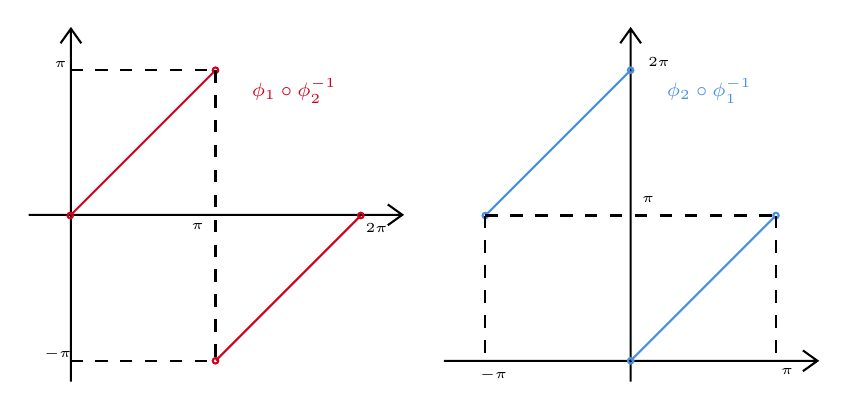
\begin{tikzpicture}[x=0.75pt,y=0.75pt,yscale=-1,xscale=1]
		%uncomment if require: \path (0,300); %set diagram left start at 0, and has height of 300
		
		%Shape: Axis 2D [id:dp031269396086308854] 
		\draw  (180,189.67) -- (360,189.67)(200.33,100) -- (200.33,270) (353,184.67) -- (360,189.67) -- (353,194.67) (195.33,107) -- (200.33,100) -- (205.33,107)  ;
		%Straight Lines [id:da8173483474090752] 
		\draw [color={rgb, 255:red, 208; green, 2; blue, 27 }  ,draw opacity=1 ][line width=0.75]    (200.24,189.76) -- (269.76,120.24) ;
		\draw [shift={(270,120)}, rotate = 315] [color={rgb, 255:red, 208; green, 2; blue, 27 }  ,draw opacity=1 ][line width=0.75]      (0, 0) circle [x radius= 1.34, y radius= 1.34]   ;
		\draw [shift={(200,190)}, rotate = 315] [color={rgb, 255:red, 208; green, 2; blue, 27 }  ,draw opacity=1 ][line width=0.75]      (0, 0) circle [x radius= 1.34, y radius= 1.34]   ;
		%Straight Lines [id:da7972743834901372] 
		\draw [color={rgb, 255:red, 208; green, 2; blue, 27 }  ,draw opacity=1 ][line width=0.75]    (270.24,259.76) -- (339.76,190.24) ;
		\draw [shift={(340,190)}, rotate = 315] [color={rgb, 255:red, 208; green, 2; blue, 27 }  ,draw opacity=1 ][line width=0.75]      (0, 0) circle [x radius= 1.34, y radius= 1.34]   ;
		\draw [shift={(270,260)}, rotate = 315] [color={rgb, 255:red, 208; green, 2; blue, 27 }  ,draw opacity=1 ][line width=0.75]      (0, 0) circle [x radius= 1.34, y radius= 1.34]   ;
		%Straight Lines [id:da11749218813373297] 
		\draw  [dash pattern={on 4.5pt off 4.5pt}]  (270,120) -- (270,260) ;
		%Shape: Axis 2D [id:dp7242837319994968] 
		\draw  (380,260) -- (560,260)(470,100) -- (470,270) (553,255) -- (560,260) -- (553,265) (465,107) -- (470,100) -- (475,107)  ;
		%Straight Lines [id:da7954245800299584] 
		\draw [color={rgb, 255:red, 74; green, 144; blue, 226 }  ,draw opacity=1 ][line width=0.75]    (400.24,189.76) -- (469.76,120.24) ;
		\draw [shift={(470,120)}, rotate = 315] [color={rgb, 255:red, 74; green, 144; blue, 226 }  ,draw opacity=1 ][line width=0.75]      (0, 0) circle [x radius= 1.34, y radius= 1.34]   ;
		\draw [shift={(400,190)}, rotate = 315] [color={rgb, 255:red, 74; green, 144; blue, 226 }  ,draw opacity=1 ][line width=0.75]      (0, 0) circle [x radius= 1.34, y radius= 1.34]   ;
		%Straight Lines [id:da15608839189923596] 
		\draw [color={rgb, 255:red, 74; green, 144; blue, 226 }  ,draw opacity=1 ][line width=0.75]    (470.24,259.76) -- (539.76,190.24) ;
		\draw [shift={(540,190)}, rotate = 315] [color={rgb, 255:red, 74; green, 144; blue, 226 }  ,draw opacity=1 ][line width=0.75]      (0, 0) circle [x radius= 1.34, y radius= 1.34]   ;
		\draw [shift={(470,260)}, rotate = 315] [color={rgb, 255:red, 74; green, 144; blue, 226 }  ,draw opacity=1 ][line width=0.75]      (0, 0) circle [x radius= 1.34, y radius= 1.34]   ;
		%Straight Lines [id:da8863860410352722] 
		\draw  [dash pattern={on 4.5pt off 4.5pt}]  (400,190) -- (400,260) ;
		%Straight Lines [id:da8092780134149673] 
		\draw  [dash pattern={on 4.5pt off 4.5pt}]  (540,190) -- (540,260) ;
		%Straight Lines [id:da9907647632614371] 
		\draw  [dash pattern={on 4.5pt off 4.5pt}]  (400,190) -- (540,190) ;
		%Straight Lines [id:da6719155425075689] 
		\draw  [dash pattern={on 4.5pt off 4.5pt}]  (200,260) -- (270,260) ;
		%Straight Lines [id:da26461137148185054] 
		\draw  [dash pattern={on 4.5pt off 4.5pt}]  (200,120) -- (270,120) ;
		
		% Text Node
		\draw (257,192.4) node [anchor=north west][inner sep=0.75pt]  [font=\tiny]  {$\pi $};
		% Text Node
		\draw (286,122.4) node [anchor=north west][inner sep=0.75pt]  [font=\scriptsize,color={rgb, 255:red, 208; green, 2; blue, 27 }  ,opacity=1 ]  {$\phi _{1} \circ \phi _{2}^{-1}$};
		% Text Node
		\draw (341,192.4) node [anchor=north west][inner sep=0.75pt]  [font=\tiny]  {$2\pi $};
		% Text Node
		\draw (396,262.4) node [anchor=north west][inner sep=0.75pt]  [font=\tiny]  {$-\pi $};
		% Text Node
		\draw (486,122.4) node [anchor=north west][inner sep=0.75pt]  [font=\scriptsize,color={rgb, 255:red, 74; green, 144; blue, 226 }  ,opacity=1 ]  {$\phi _{2} \circ \phi _{1}^{-1}$};
		% Text Node
		\draw (541,262.4) node [anchor=north west][inner sep=0.75pt]  [font=\tiny]  {$\pi $};
		% Text Node
		\draw (474,179.4) node [anchor=north west][inner sep=0.75pt]  [font=\tiny]  {$\pi $};
		% Text Node
		\draw (477,112.4) node [anchor=north west][inner sep=0.75pt]  [font=\tiny]  {$2\pi $};
		% Text Node
		\draw (191,114.4) node [anchor=north west][inner sep=0.75pt]  [font=\tiny]  {$\pi $};
		% Text Node
		\draw (186,252.4) node [anchor=north west][inner sep=0.75pt]  [font=\tiny]  {$-\pi $};
		
		
	\end{tikzpicture}
\end{figure}
	
\end{solution}

\begin{observation}
	I was thinking about my solution to the problem above, and I thought it is wrong, as I was thinking that the function $ \phi_1 $ is not homeomorphism as it is not continuous. But the point that I was missing is that this function is indeed continuous on its domain and the point of discontinuity (i.e. $ x = \pi $) is not in the domain. 
\end{observation}

\begin{problem}{Another $ C^\infty $ atlas on a circle}
	\label{problem:S^1Charts}
	In the previous problem, we constructed an atlas for a unit circle siting in the complex plane. In this problem we are going to construct a different atlas for a unit circle siting in the $ x-y $ plane. The following diagram are the charts for this unit circle. Write these charts explicitly and check if they are pairwise compatible.
	\begin{figure}[h!]
	
	
	\centering
	\tikzset{every picture/.style={line width=0.75pt}} %set default line width to 0.75pt        
	
	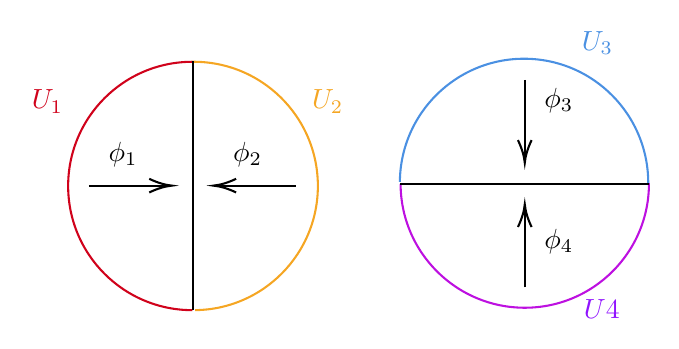
\begin{tikzpicture}[x=0.75pt,y=0.75pt,yscale=-1,xscale=1]
		%uncomment if require: \path (0,300); %set diagram left start at 0, and has height of 300
		
		%Shape: Arc [id:dp023481932229717062] 
		\draw  [draw opacity=0] (199.83,250) .. controls (199.83,250) and (199.83,250) .. (199.83,250) .. controls (199.83,250) and (199.83,250) .. (199.83,250) .. controls (166.79,250) and (140,223.21) .. (140,190.17) .. controls (140,157.12) and (166.79,130.33) .. (199.83,130.33) -- (199.83,190.17) -- cycle ; \draw  [color={rgb, 255:red, 208; green, 2; blue, 27 }  ,draw opacity=1 ] (199.83,250) .. controls (199.83,250) and (199.83,250) .. (199.83,250) .. controls (199.83,250) and (199.83,250) .. (199.83,250) .. controls (166.79,250) and (140,223.21) .. (140,190.17) .. controls (140,157.12) and (166.79,130.33) .. (199.83,130.33) ;  
		%Shape: Arc [id:dp8279857043077765] 
		\draw  [draw opacity=0] (199.83,130.33) .. controls (199.83,130.33) and (199.83,130.33) .. (199.83,130.33) .. controls (232.88,129.98) and (259.95,156.47) .. (260.31,189.52) .. controls (260.67,222.56) and (234.17,249.64) .. (201.13,249.99) -- (200.48,190.16) -- cycle ; \draw  [color={rgb, 255:red, 245; green, 166; blue, 35 }  ,draw opacity=1 ] (199.83,130.33) .. controls (199.83,130.33) and (199.83,130.33) .. (199.83,130.33) .. controls (232.88,129.98) and (259.95,156.47) .. (260.31,189.52) .. controls (260.67,222.56) and (234.17,249.64) .. (201.13,249.99) ;  
		%Shape: Arc [id:dp2277450931666709] 
		\draw  [draw opacity=0] (299.82,188.21) .. controls (299.82,188.21) and (299.82,188.21) .. (299.82,188.21) .. controls (300.08,155.16) and (327.08,128.59) .. (360.13,128.86) .. controls (393.17,129.12) and (419.75,156.12) .. (419.48,189.17) -- (359.65,188.69) -- cycle ; \draw  [color={rgb, 255:red, 74; green, 144; blue, 226 }  ,draw opacity=1 ] (299.82,188.21) .. controls (299.82,188.21) and (299.82,188.21) .. (299.82,188.21) .. controls (300.08,155.16) and (327.08,128.59) .. (360.13,128.86) .. controls (393.17,129.12) and (419.75,156.12) .. (419.48,189.17) ;  
		%Shape: Arc [id:dp16056893747855794] 
		\draw  [draw opacity=0] (419.83,188.83) .. controls (419.83,188.83) and (419.83,188.83) .. (419.83,188.83) .. controls (419.93,221.88) and (393.21,248.74) .. (360.17,248.83) .. controls (327.12,248.93) and (300.26,222.21) .. (300.17,189.17) -- (360,189) -- cycle ; \draw  [color={rgb, 255:red, 189; green, 16; blue, 224 }  ,draw opacity=1 ] (419.83,188.83) .. controls (419.83,188.83) and (419.83,188.83) .. (419.83,188.83) .. controls (419.93,221.88) and (393.21,248.74) .. (360.17,248.83) .. controls (327.12,248.93) and (300.26,222.21) .. (300.17,189.17) ;  
		%Straight Lines [id:da9947609889928073] 
		\draw    (150,190) -- (188,190) ;
		\draw [shift={(190,190)}, rotate = 180] [color={rgb, 255:red, 0; green, 0; blue, 0 }  ][line width=0.75]    (10.93,-3.29) .. controls (6.95,-1.4) and (3.31,-0.3) .. (0,0) .. controls (3.31,0.3) and (6.95,1.4) .. (10.93,3.29)   ;
		%Straight Lines [id:da6553860547904606] 
		\draw    (212,190) -- (250,190) ;
		\draw [shift={(210,190)}, rotate = 0] [color={rgb, 255:red, 0; green, 0; blue, 0 }  ][line width=0.75]    (10.93,-3.29) .. controls (6.95,-1.4) and (3.31,-0.3) .. (0,0) .. controls (3.31,0.3) and (6.95,1.4) .. (10.93,3.29)   ;
		%Straight Lines [id:da19474028508083085] 
		\draw    (360,139) -- (360,177) ;
		\draw [shift={(360,179)}, rotate = 270] [color={rgb, 255:red, 0; green, 0; blue, 0 }  ][line width=0.75]    (10.93,-3.29) .. controls (6.95,-1.4) and (3.31,-0.3) .. (0,0) .. controls (3.31,0.3) and (6.95,1.4) .. (10.93,3.29)   ;
		%Straight Lines [id:da648683487634115] 
		\draw    (360,239) -- (360,201) ;
		\draw [shift={(360,199)}, rotate = 90] [color={rgb, 255:red, 0; green, 0; blue, 0 }  ][line width=0.75]    (10.93,-3.29) .. controls (6.95,-1.4) and (3.31,-0.3) .. (0,0) .. controls (3.31,0.3) and (6.95,1.4) .. (10.93,3.29)   ;
		%Straight Lines [id:da9130830416071034] 
		\draw    (200,130) -- (200,250) ;
		%Straight Lines [id:da1322223309435544] 
		\draw    (420,189) -- (300,189) ;
		
		% Text Node
		\draw (121,142.4) node [anchor=north west][inner sep=0.75pt]  [color={rgb, 255:red, 208; green, 2; blue, 27 }  ,opacity=1 ]  {$U_{1}$};
		% Text Node
		\draw (256,142.4) node [anchor=north west][inner sep=0.75pt]  [color={rgb, 255:red, 245; green, 166; blue, 35 }  ,opacity=1 ]  {$U_{2}$};
		% Text Node
		\draw (386,114.4) node [anchor=north west][inner sep=0.75pt]  [color={rgb, 255:red, 74; green, 144; blue, 226 }  ,opacity=1 ]  {$U_{3}$};
		% Text Node
		\draw (387,243.4) node [anchor=north west][inner sep=0.75pt]  [color={rgb, 255:red, 144; green, 19; blue, 254 }  ,opacity=1 ]  {$U4$};
		% Text Node
		\draw (158,167.4) node [anchor=north west][inner sep=0.75pt]    {$\phi _{1}$};
		% Text Node
		\draw (218,167.4) node [anchor=north west][inner sep=0.75pt]    {$\phi _{2}$};
		% Text Node
		\draw (368,141.4) node [anchor=north west][inner sep=0.75pt]    {$\phi _{3}$};
		% Text Node
		\draw (368,209.4) node [anchor=north west][inner sep=0.75pt]    {$\phi _{4}$};
		
		
	\end{tikzpicture}
\end{figure}

\FloatBarrier
\end{problem}
\begin{solution}
	The explicit formulas for the charts depicted above is as following
	\[ (U_1, \phi_1:U_1\to \R),(U_2, \phi_2:U_2\to \R), (U_3, \phi_3:U_3\to \R),(U_4, \phi_4:U_4\to \R), \]
	where we have
	\[ \phi_1(x,y) = y,\qquad  \phi_2(x,y) = y, \qquad \phi_3(x,y) = x, \qquad \phi_4(x,y) = x. \]
	Note that although some of the functions above might have a same formula, but they are different functions as they have different domains. To show that these functions are pairwise compatible, we start by noting that since $ U_1 \cap U_2 = \emptyset $, thus $ (U_1,\phi_1) $ and $ (U_2,\phi_2) $ are compatible. With the same reasoning, the charts $ (U_3,\phi_3) $ and $ (U_4,\phi_4) $ are compatible. Now, we want to show that $ (U_1,\phi_1) $ is compatible with $ (U_3,\phi_3) $. We need to show that 
	\[ \phi_1 \circ \inv{\phi_3}: \underbrace{\phi_3(U_1\cap U_3)}_{(-1,0)} \to \underbrace{\phi_1(U_1\cap U_3)}_{(0,1)}\quad \text{and} \quad \phi_3\circ \inv{\phi_1}:\underbrace{\phi_1(U_1\cap U_3)}_{(0,1)} \to \underbrace{\phi_3(U_1\cap  U_3)}_{(-1,0)} \]
	are $ C^\infty $. To write them explicitly, we have
	\[ (\phi_1 \circ \inv{\phi_3})(x) = \phi_1(x,\sqrt{1-x^2}) = \sqrt{1-x^2}.  \]
	Also
	\[ (\phi_3 \circ \inv{\phi_1})(x) = \phi_3(-\sqrt{1-x^2},x) = -\sqrt{1-x^2}. \]
	We can see that both of these functions are $ C^\infty $ in their domain. Now, for the charts $ (U_1, \phi_1) $ and $ (U_4,\phi_4) $ need to show
	\[ \phi_1 \circ \inv{\phi_4}:\underbrace{ \phi_4(U_1\cap U_4)}_{(-1,0)} \to \underbrace{\phi_1(U_1\cap U_4)}_{(-1,0)} \qquad \text{and} \qquad \phi_4\circ \inv{\phi_1}: \underbrace{\phi_1(U_1\cap U_4)}_{(-1,0)} \to  \underbrace{\phi_4(U_1\cap U_4)}_{(-1,0)} \]
	are $ C^\infty $ in their domain. Explicitly, we have
	\[ (\phi_1 \circ \inv{\phi_4})(x) = -\sqrt{1 -x^2}, \qquad (\phi_4\circ \inv{\phi_1})(x) = -\sqrt{1-x^2}.\]
	With the same strategy, we can show that this collection of charts indeed makes a $ C^\infty $ atlas for the unit circle in $ x-y $ plane.
\end{solution}


\begin{problem}[The real line with two origins (from W. Tu)]
	Let $ A $ and $ B $ be two points not on the real line $ \R $. Consider the set $ S = (\R - \set{0}) \cup \set{A,B} $. For nay two positive real numbers $ c,d $, define 
	\[ I_A(-c,d) = (-c,0) \cup \set{A} \cap (0,d) \]
	and similarly for $ I_B(-c,d) $, with $ B $ instead of $ A $. Define a topology on $ S $ as follows: On $ (\R - \set{0}) $, use the subspace topology inherited from $ \R $, with open intervals as a basis. A basis of neighborhoods at $ A $ is the set $ \set{I_A(-c,d)\ |\ c,d > 0} $; similarly, a basis of neighborhoods at $ B $ is $ \set{I_B(-c,d)\ |\ c,d > 0} $.
	\begin{enumerate}[(a)]
		\item Prove that the map $ h: I_A(-c,d) \to (-c,d) $ defined by
		\begin{align*}
			h(x)&=x \qquad \text{for}\ x\in(-c,0) \cup (0,d),\\
			h(A)&=0
		\end{align*}
		is a homeomorphism.
		
		\item Show that $ S $ is locally Euclidean and second countable, but not Hausdorff.
	\end{enumerate}
\end{problem}

\begin{solution}
	\begin{enumerate}[(a)]
		\item We need to show that $ h $ is one-to-one, onto, and continuous, with continuous inverse. To show being one-to-one, let $ x,y \in I_A(-c,d) $ such that $ x\neq y $ and possibly one of them equal to $ A $. If none is equal to $ A $, then $ h $ is the identity map which is one-to-one. However, if one of them is equal to $ A $, let's say $ x = A $, then $ h(x) = 0 $ where $ h(y) \in (-c,d)\cup(0,d)$, thus $ h(y) \neq 0 $. This proves that $ h $ is indeed one to one. To show that the function is onto, let $ z \in (-c,d) $. Then if $ z = 0 $ we have $ h(A) = z $, and if $ z \neq 0 $, we have $ h(z) = z $. Thus the function $ h $ is a bijection.
		
		As the second step, we need to show that this function is continuous with continuous inverse. From definition of continuoity, we just need to show that both $ h $ and $ \inv{h} $ maps opens to opens (because for continuous function the pre-image of every open set is an open set; and to show that the inverse of the function is also continuous we need to show that the image of every open is also open).
		Let $ U = (a,b) \subset I_A(-c,d) $ be an open set in the topology of $ S $. If $ A \notin (a,b) $, then the image of this set under $ h $ is $ (a,b) $ which is open in $ (-c,d) $. But if $ A \in (a,b) $, then the image of this set under the map $ h $ is $ (a,0)\cup(0,b)\cup\set{0} = (a,b) $, which is also open. Thus $ \inv{h} $ is continuous. To show the continuity of $ \inv{h} $, let $ (a,b) \subset (c,d) $. If $ 0 \notin (a,b) $, then pre-image of this set under the map $ f $ is $ (a,b) $ that is open in $ S $. However if $ 0 \in (a,b) $, then the pre-image of this set under $ f $ is the set $ (-a,0) \cup \set{A} \cup (0,b) $ which is indeed open in $ S $ as we can construct this with the basis if opens at $ A $.
		
		\item First, we show that $ S $ is locally Euclidean. To show this let $ p \in S $. If $ p \neq A $ and $ p \neq B $, then we choose an open set $ U =  (a,b) $ containing $ p $ that does not contain neither of $ A $ and  $ B $. Then $ U $ is homeomorphic to $ (a,b) $ with the identity map. However if $ p = A $, we choose any open $ U = (a,b) $ containing $ p $. Then $ (U = (a,b),I_A(a,b)) $ is a local chart. For the case where $ p = B $, we can find a suitable chart with the same reasoning as for $ A $. Thus we have shown that $ S $ is locally Euclidean.
		
		To show that $ S $ is second countable, let $ \mathcal{B} $ be a basis for $ \R - \set{0} $. Since $ \R $ is second countable, then $ \mathcal{B} $ is countable. Let $ \mathbb{B} = \mathcal{B} \cup I_A(-c,d) \cup I_B(-c,d) $ is a countable basis for $ S $ for some $ c,d > 0 $. This shows that $ S $ is also second countable.
		
		However, this space is not Hausdorff. To show this consider the points $ A,B $. We can not find any two open $ U,V $ such that $ A \in U $ and $ B \in V $ and we have $ U \cap V = \emptyset $. Or equivalently, for all open sets $ U,V $  such that $ A \in U $ and $ B \in V $ we have $ U\cap V \neq \emptyset $. That is because from the basis of the open neighborhoods at $ A,B $ we have $ U = I_A(-c,d) $ and $ V = I_B(-e,f) $ for some $ c,d,e,f > 0 $. It is clear that $ U \cap V \neq 0 $, thus $ S $ is not Hausdorff.
	\end{enumerate}
\end{solution}

\begin{problem}[A sphere with a hair (from W. Tu) ] 
	A fundamental theorem of topology, the theorem on invariance of dimension, states that if two nonempty open sets $ U \subset \R^n $ and $ V \subset \R^m $ are homeomorphic, then $ n = m $. Prove that the sphere with a hair in $ \R^3 $ is not locally Euclidean at $ q $ (the point that the hair attaches to the sphere). Hence it cannot be a topological manifold. 
\end{problem}

\begin{solution}
	We will proceed with the proof by contradiction. Assume that the ball with hair at  point $ q $ is homeomorphic to some open set in $ \R^n $. Then $ q $ has an open neighborhood $ U $ homeomorphic to an open ball $ B := \mathbb{B}(0,\epsilon) \in \R^n $, with $ q $ mapping to 0. We can restrict this homeomorphism to a homeomorphism $ U - \set{q} \to B - \set{0} $. Now $ B-\set{0} $ is either connected if $ n \geq 2 $ or has two connected components if $ n=1 $, where $ U - \set{q} $ has two connected components where one component is a 1 dimensional manifold (the hair) and the other component is a 2 dimensional manifold (the sphere). The only case where $ B - \set{0} $ has two connected components is when $ n = 1 $. But because of the invariance of dimension principle, the sphere (2 dimensional manifold) can not be homeomorphic to a one dimensional manifold. Thus there is no such a homeomorphism between the hairy ball and $ \R^n $ and the hairy ball is not locally Euclidean in $ q $.
\end{solution}

\begin{problem}[Charts on a sphere (from W. Tu)]
	Let $ S^2 $ be the unit sphere, i.e.
	\[ S^2 = \set{(x,y,z)\in\R^3\ :\ x^2+y^2+z^2 = 1} \]
	in $ \R^3 $. Define in $ S^2 $ the six charts corresponding to the six hemispheres (from the front, rear, right, left, upper, and lower hemispheres) as in the figure.
	\begin{align*}
		U_1 = \set{(x,y,z) \in S^2\ |\ x > 0}, \qquad \phi_1(x,y,z) = (y,z), \\
		U_2 = \set{(x,y,z) \in S^2\ |\ x < 0}, \qquad \phi_2(x,y,z) = (y,z), \\
		U_3 = \set{(x,y,z) \in S^2\ |\ y > 0}, \qquad \phi_3(x,y,z) = (x,z), \\
		U_4 = \set{(x,y,z) \in S^2\ |\ y < 0}, \qquad \phi_4(x,y,z) = (x,z), \\
		U_5 = \set{(x,y,z) \in S^2\ |\ z > 0}, \qquad \phi_5(x,y,z) = (x,y), \\
		U_6 = \set{(x,y,z) \in S^2\ |\ z < 0}, \qquad \phi_6(x,y,z) = (x,y).
	\end{align*}
	Note that although some of the functions above might look similar (like $ \phi_3 $ and $ \phi_4 $) but they are in fact different functions as they have different domains. Show that $ \phi_1\circ \inv{\phi_4}, \phi_4 \circ \inv{\phi_1} $ is $ C^\infty $ on $ \phi_4(U_1 \cap U_4), \phi_1(U_1 \cap U_4) $ respectively. Do the same same analysis for $ \phi_6 \circ \inv{\phi_1}$.
	\begin{figure}[h!]
	
	\centering
	
	\tikzset{every picture/.style={line width=0.75pt}} %set default line width to 0.75pt        
	
	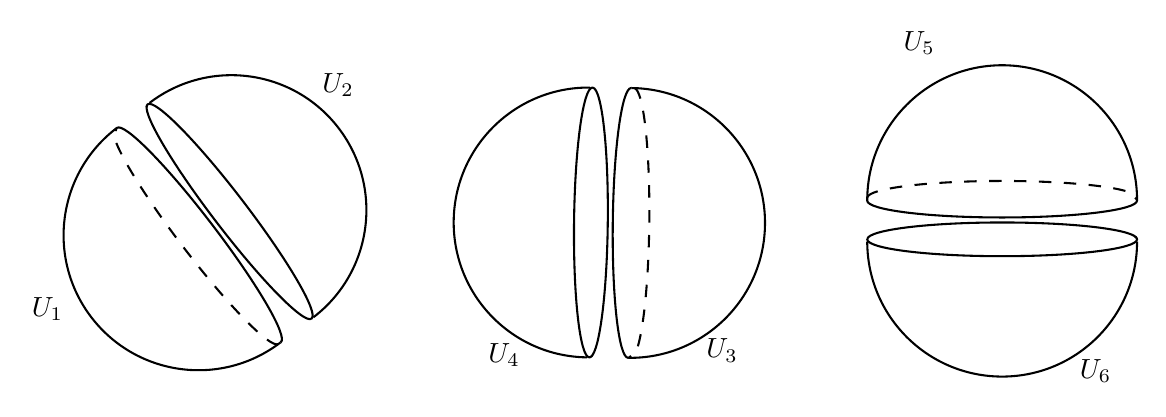
\begin{tikzpicture}[x=0.75pt,y=0.75pt,yscale=-1,xscale=1]
		%uncomment if require: \path (0,300); %set diagram left start at 0, and has height of 300
		
		%Shape: Arc [id:dp8087392079745468] 
		\draw  [draw opacity=0] (610,205) .. controls (610,205) and (610,205) .. (610,205) .. controls (610,240.9) and (580.9,270) .. (545,270) .. controls (509.1,270) and (480,240.9) .. (480,205) -- (545,205) -- cycle ; \draw   (610,205) .. controls (610,205) and (610,205) .. (610,205) .. controls (610,240.9) and (580.9,270) .. (545,270) .. controls (509.1,270) and (480,240.9) .. (480,205) ;  
		%Shape: Arc [id:dp7144643582066421] 
		\draw  [draw opacity=0] (480.02,203.67) .. controls (480.89,199.28) and (509.65,195.75) .. (545,195.75) .. controls (578.58,195.75) and (606.22,198.93) .. (609.64,203.02) -- (545,203.88) -- cycle ; \draw   (480.02,203.67) .. controls (480.89,199.28) and (509.65,195.75) .. (545,195.75) .. controls (578.58,195.75) and (606.22,198.93) .. (609.64,203.02) ;  
		%Shape: Arc [id:dp9774877190814104] 
		\draw  [draw opacity=0] (480,185) .. controls (480,185) and (480,185) .. (480,185) .. controls (480,149.1) and (509.1,120) .. (545,120) .. controls (580.9,120) and (610,149.1) .. (610,185) -- (545,185) -- cycle ; \draw   (480,185) .. controls (480,185) and (480,185) .. (480,185) .. controls (480,149.1) and (509.1,120) .. (545,120) .. controls (580.9,120) and (610,149.1) .. (610,185) ;  
		%Shape: Arc [id:dp7118645098131682] 
		\draw  [draw opacity=0] (609.09,202.51) .. controls (609.69,202.95) and (610,203.41) .. (610,203.88) .. controls (610,208.36) and (580.9,212) .. (545,212) .. controls (509.1,212) and (480,208.36) .. (480,203.88) .. controls (480,203.8) and (480.01,203.73) .. (480.02,203.66) -- (545,203.88) -- cycle ; \draw   (609.09,202.51) .. controls (609.69,202.95) and (610,203.41) .. (610,203.88) .. controls (610,208.36) and (580.9,212) .. (545,212) .. controls (509.1,212) and (480,208.36) .. (480,203.88) .. controls (480,203.8) and (480.01,203.73) .. (480.02,203.66) ;  
		%Shape: Arc [id:dp7962209595423704] 
		\draw  [draw opacity=0] (609.06,183.85) .. controls (609.66,184.29) and (609.98,184.75) .. (609.98,185.22) .. controls (609.98,189.7) and (580.88,193.34) .. (544.98,193.34) .. controls (509.08,193.34) and (479.98,189.7) .. (479.98,185.22) .. controls (479.98,185.14) and (479.99,185.07) .. (480,185) -- (544.98,185.22) -- cycle ; \draw   (609.06,183.85) .. controls (609.66,184.29) and (609.98,184.75) .. (609.98,185.22) .. controls (609.98,189.7) and (580.88,193.34) .. (544.98,193.34) .. controls (509.08,193.34) and (479.98,189.7) .. (479.98,185.22) .. controls (479.98,185.14) and (479.99,185.07) .. (480,185) ;  
		%Shape: Arc [id:dp26854896682720364] 
		\draw  [draw opacity=0][dash pattern={on 4.5pt off 4.5pt}] (480.02,183.67) .. controls (480.89,179.28) and (509.65,175.75) .. (545,175.75) .. controls (578.58,175.75) and (606.22,178.93) .. (609.64,183.02) -- (545,183.88) -- cycle ; \draw  [dash pattern={on 4.5pt off 4.5pt}] (480.02,183.67) .. controls (480.89,179.28) and (509.65,175.75) .. (545,175.75) .. controls (578.58,175.75) and (606.22,178.93) .. (609.64,183.02) ;  
		%Shape: Arc [id:dp8593027572319052] 
		\draw  [draw opacity=0] (345,260.74) .. controls (345,260.74) and (345,260.74) .. (345,260.74) .. controls (345,260.74) and (345,260.74) .. (345,260.74) .. controls (309.1,260.33) and (280.34,230.89) .. (280.75,195) .. controls (281.16,159.1) and (310.6,130.34) .. (346.49,130.75) -- (345.74,195.74) -- cycle ; \draw   (345,260.74) .. controls (345,260.74) and (345,260.74) .. (345,260.74) .. controls (345,260.74) and (345,260.74) .. (345,260.74) .. controls (309.1,260.33) and (280.34,230.89) .. (280.75,195) .. controls (281.16,159.1) and (310.6,130.34) .. (346.49,130.75) ;  
		%Shape: Arc [id:dp5017110012711772] 
		\draw  [draw opacity=0] (347.82,130.78) .. controls (352.2,131.7) and (355.4,160.5) .. (354.99,195.85) .. controls (354.61,229.43) and (351.11,257.03) .. (346.98,260.41) -- (346.87,195.76) -- cycle ; \draw   (347.82,130.78) .. controls (352.2,131.7) and (355.4,160.5) .. (354.99,195.85) .. controls (354.61,229.43) and (351.11,257.03) .. (346.98,260.41) ;  
		%Shape: Arc [id:dp34022749055732393] 
		\draw  [draw opacity=0] (366.49,130.98) .. controls (366.49,130.98) and (366.49,130.98) .. (366.49,130.98) .. controls (402.39,131.39) and (431.15,160.83) .. (430.74,196.72) .. controls (430.33,232.62) and (400.89,261.38) .. (364.99,260.97) -- (365.74,195.97) -- cycle ; \draw   (366.49,130.98) .. controls (366.49,130.98) and (366.49,130.98) .. (366.49,130.98) .. controls (402.39,131.39) and (431.15,160.83) .. (430.74,196.72) .. controls (430.33,232.62) and (400.89,261.38) .. (364.99,260.97) ;  
		%Shape: Arc [id:dp9156415467589833] 
		\draw  [draw opacity=0] (347.5,259.86) .. controls (347.05,260.45) and (346.59,260.76) .. (346.12,260.75) .. controls (341.63,260.7) and (338.33,231.56) .. (338.74,195.66) .. controls (339.16,159.77) and (343.13,130.71) .. (347.62,130.76) .. controls (347.69,130.76) and (347.76,130.77) .. (347.83,130.79) -- (346.87,195.76) -- cycle ; \draw   (347.5,259.86) .. controls (347.05,260.45) and (346.59,260.76) .. (346.12,260.75) .. controls (341.63,260.7) and (338.33,231.56) .. (338.74,195.66) .. controls (339.16,159.77) and (343.13,130.71) .. (347.62,130.76) .. controls (347.69,130.76) and (347.76,130.77) .. (347.83,130.79) ;  
		%Shape: Arc [id:dp7534866185784517] 
		\draw  [draw opacity=0] (366.15,260.05) .. controls (365.7,260.64) and (365.24,260.95) .. (364.78,260.95) .. controls (360.29,260.89) and (356.99,231.75) .. (357.4,195.86) .. controls (357.82,159.96) and (361.79,130.9) .. (366.28,130.95) .. controls (366.35,130.96) and (366.42,130.96) .. (366.49,130.98) -- (365.53,195.95) -- cycle ; \draw   (366.15,260.05) .. controls (365.7,260.64) and (365.24,260.95) .. (364.78,260.95) .. controls (360.29,260.89) and (356.99,231.75) .. (357.4,195.86) .. controls (357.82,159.96) and (361.79,130.9) .. (366.28,130.95) .. controls (366.35,130.96) and (366.42,130.96) .. (366.49,130.98) ;  
		%Shape: Arc [id:dp7058755896129407] 
		\draw  [draw opacity=0][dash pattern={on 4.5pt off 4.5pt}] (367.82,131.01) .. controls (372.2,131.93) and (375.4,160.73) .. (374.99,196.08) .. controls (374.61,229.66) and (371.1,257.26) .. (366.98,260.64) -- (366.87,195.99) -- cycle ; \draw  [dash pattern={on 4.5pt off 4.5pt}] (367.82,131.01) .. controls (372.2,131.93) and (375.4,160.73) .. (374.99,196.08) .. controls (374.61,229.66) and (371.1,257.26) .. (366.98,260.64) ;  
		%Shape: Arc [id:dp6580687340920708] 
		\draw  [draw opacity=0] (134.21,138.15) .. controls (134.21,138.15) and (134.21,138.15) .. (134.21,138.15) .. controls (134.21,138.15) and (134.21,138.15) .. (134.21,138.15) .. controls (162.73,116.35) and (203.52,121.79) .. (225.32,150.31) .. controls (247.13,178.82) and (241.69,219.62) .. (213.17,241.42) -- (173.69,189.79) -- cycle ; \draw   (134.21,138.15) .. controls (134.21,138.15) and (134.21,138.15) .. (134.21,138.15) .. controls (134.21,138.15) and (134.21,138.15) .. (134.21,138.15) .. controls (162.73,116.35) and (203.52,121.79) .. (225.32,150.31) .. controls (247.13,178.82) and (241.69,219.62) .. (213.17,241.42) ;  
		%Shape: Arc [id:dp04807301977746614] 
		\draw  [draw opacity=0] (212.1,242.21) .. controls (208.08,244.19) and (187.81,223.49) .. (166.34,195.4) .. controls (145.94,168.73) and (131.69,144.84) .. (132.85,139.64) -- (172.79,190.47) -- cycle ; \draw   (212.1,242.21) .. controls (208.08,244.19) and (187.81,223.49) .. (166.34,195.4) .. controls (145.94,168.73) and (131.69,144.84) .. (132.85,139.64) ;  
		%Shape: Arc [id:dp5373023961242778] 
		\draw  [draw opacity=0] (197.28,253.57) .. controls (197.28,253.57) and (197.28,253.57) .. (197.28,253.57) .. controls (197.28,253.57) and (197.28,253.57) .. (197.28,253.57) .. controls (168.76,275.37) and (127.97,269.93) .. (106.16,241.41) .. controls (84.36,212.89) and (89.8,172.1) .. (118.32,150.3) -- (157.8,201.93) -- cycle ; \draw   (197.28,253.57) .. controls (197.28,253.57) and (197.28,253.57) .. (197.28,253.57) .. controls (197.28,253.57) and (197.28,253.57) .. (197.28,253.57) .. controls (168.76,275.37) and (127.97,269.93) .. (106.16,241.41) .. controls (84.36,212.89) and (89.8,172.1) .. (118.32,150.3) ;  
		%Shape: Arc [id:dp6075301311311689] 
		\draw  [draw opacity=0] (132.79,140.39) .. controls (132.77,139.64) and (132.95,139.11) .. (133.31,138.83) .. controls (136.88,136.11) and (157.44,157.02) .. (179.25,185.53) .. controls (201.05,214.05) and (215.84,239.38) .. (212.27,242.11) .. controls (212.22,242.15) and (212.15,242.19) .. (212.09,242.22) -- (172.79,190.47) -- cycle ; \draw   (132.79,140.39) .. controls (132.77,139.64) and (132.95,139.11) .. (133.31,138.83) .. controls (136.88,136.11) and (157.44,157.02) .. (179.25,185.53) .. controls (201.05,214.05) and (215.84,239.38) .. (212.27,242.11) .. controls (212.22,242.15) and (212.15,242.19) .. (212.09,242.22) ;  
		%Shape: Arc [id:dp4893987696896971] 
		\draw  [draw opacity=0] (117.98,151.74) .. controls (117.96,150.99) and (118.14,150.47) .. (118.5,150.18) .. controls (122.07,147.46) and (142.64,168.37) .. (164.44,196.89) .. controls (186.24,225.4) and (201.03,250.73) .. (197.46,253.46) .. controls (197.41,253.5) and (197.34,253.54) .. (197.28,253.57) -- (157.98,201.82) -- cycle ; \draw   (117.98,151.74) .. controls (117.96,150.99) and (118.14,150.47) .. (118.5,150.18) .. controls (122.07,147.46) and (142.64,168.37) .. (164.44,196.89) .. controls (186.24,225.4) and (201.03,250.73) .. (197.46,253.46) .. controls (197.41,253.5) and (197.34,253.54) .. (197.28,253.57) ;  
		%Shape: Arc [id:dp5010740042347757] 
		\draw  [draw opacity=0][dash pattern={on 4.5pt off 4.5pt}] (196.21,254.36) .. controls (192.19,256.34) and (171.92,235.64) .. (150.45,207.55) .. controls (130.05,180.87) and (115.8,156.99) .. (116.96,151.78) -- (156.91,202.62) -- cycle ; \draw  [dash pattern={on 4.5pt off 4.5pt}] (196.21,254.36) .. controls (192.19,256.34) and (171.92,235.64) .. (150.45,207.55) .. controls (130.05,180.87) and (115.8,156.99) .. (116.96,151.78) ;  
		
		% Text Node
		\draw (76,230.4) node [anchor=north west][inner sep=0.75pt]    {$U_{1}$};
		% Text Node
		\draw (216,122.4) node [anchor=north west][inner sep=0.75pt]    {$U_{2}$};
		% Text Node
		\draw (401,250.4) node [anchor=north west][inner sep=0.75pt]    {$U_{3}$};
		% Text Node
		\draw (296,252.4) node [anchor=north west][inner sep=0.75pt]    {$U_{4}$};
		% Text Node
		\draw (496,102.4) node [anchor=north west][inner sep=0.75pt]    {$U_{5}$};
		% Text Node
		\draw (581,260.4) node [anchor=north west][inner sep=0.75pt]    {$U_{6}$};
		
		
	\end{tikzpicture}
\end{figure}
\end{problem}
\begin{solution}
	For the set $ U_1 \cap U_4 $ we have
	\[ U_1 \cap U_4 = \set{(x,y,z) \in S^2\ :\ x>0 \text{ and } y < 0 }. \]
	Thus we will have
	\[ \phi_4(U_1\cap U_4) = \set{(x,z)\in \R^2 \ :\ x^2 + z^2 \leq 1,\ x>0}. \]
	Thus we can write
	\[ (\phi_1 \circ \inv{\phi_4})(\langle x,z \rangle ) = \phi_1(\langle x,-\sqrt{1-(x^2+y^2)},z \rangle) = \langle -\sqrt{1-(x^2+y^2)},z \rangle  \]
	This is indeed a $ C^\infty $ vector valued function, since each component is a $ C^\infty $ function. Now to evaluate $ \phi_4 \circ \inv{\phi_1}: \phi_1(U_1 \cap U_4) \to \phi_4(U_1\cap U_4) $ we need to first evaluate the set $ \phi_1(U_1 \cap U_4) $. For this set we have
	\[ \phi_1(U_1 \cap U_4) = \set{(z,y)\in\R^2\ :\ z^2 + y^2 \leq 1, y < 0}. \]
	Then we can write
	\[ (\phi_4 \circ \inv{\phi_1})(\langle y,z \rangle ) = \phi_4(\langle \sqrt{1-(y^2+z^2)}, y,z  \rangle) = \langle \sqrt{1-(y^2+z^2)} , z \rangle. \]
	This is indeed a $ C^\infty $ vector valued function. 
	
	To evaluate the function $ \phi_6 \circ \inv{\phi}_1: \phi_1(U_1 \cap U_6) \to \phi_6(U_1 \cap U_6) $, we first need to determine the domain of this function. First observe that 
	\[ U_1 \cap U_6 =  \set{(x,y,z) \in S^2\ :\ x>0 \text{ and } y<0}, \]
	which is the same as $ U_1 \cap U_4 $. Then for the domain of the function of interest we can write
	\[ \phi_1(U_1 \cap U_6) = \set{(y,z) \in \R^2 :\ z^2 + y^2 \leq 1 \text{ and } y<0}, \]
	\[ (\phi_6 \circ \inv{\phi_1})(\langle y,z \rangle) = \phi_6(\langle \sqrt{1-(y^2+z^2)},y,z \rangle) = \langle \sqrt{1-(y^2+z^2)}, y \rangle. \]
\end{solution}

\begin{problem}[Existence of a coordinate neighborhood (from W. Tu)]
	Let $ \set{(U_\alpha, \phi_\alpha)}_{\alpha \in I} $ be the maximal atlas on manifold $ M $. For any open set $ U $ in $ M $ and a point $ p \in U $, prove the existence of a coordinate open set $ U_\alpha $ such that $ p \in U_\alpha \subset U $.
\end{problem}
\begin{solution}
	Since $ \set{(U_\alpha,\phi_\alpha)}_{\alpha \in I} $ is an atlas, then for $ p \in U $ given as above, we can find some $ \alpha_1 \in I $ such that $ p \in U_{\alpha_1} $. Consider the open set $ W = U_{\alpha_1} \cap U $. The chart $ (W, \phi_{\alpha_1}|_W) $ is in the atlas (since it is maximal), i.e. $ \exists \alpha \in I $ such that $ (U_\alpha, \phi_\alpha) = (W, \phi_{\alpha_1}|_W) $. This completes the proof.
\end{solution}

\begin{problem}[An atlas for a product manifold (from W. Tu)]
	Prove the following proposition.
	\begin{proposition}
		If $ \set{(U_\alpha,\phi_\alpha)} $ and $ \set{(V_i,\psi_i)} $ are $ C^\infty $ atlases for the manifold $ M $ and $ N $ of dimensions $ m $ and $ n $, respectively, then the collection 
		\[ \set{(U_\alpha \times V_i,\phi_\alpha \times \psi_i)} \] where
		\[ \phi_\alpha \times \psi_i\ :\ U_\alpha \times V_i \to \R^m \times \R^n \]
		of charts is a $ C^\infty $ atlas on $ M\times N $. Therefore, $ M\times N $ is a $ C^\infty $ manifold of dimension $ m+n $.
	\end{proposition}
\end{problem}
\begin{solution}
	In order to show that the collection $ \frak{U} = \set{(U_\alpha \times V_i, \phi_\alpha \times \psi_i)} $ is an atlas for $ M\times N $, we need to show that charts are pairwise compatible as well as the set covering the whole space. To show that the chart covers the whole space $ M\times N $, let $ (p_1,p_2) \in M\times N $. Then $ p_1 \in M $ and $ p_2 \in N $. Then there are two coordinate open sets such that $ p_1 \in U_{\alpha_1} $ and $ p_2 \in V_{i_1} $. Thus the coordinate open set $ U_{\alpha_1} \times V_{i_1} $ contains the point $ (p_1,p_2) $.
	
	To show that two any two charts in the collection $ \frak{U} $ are compatible, let $ (U_{\alpha_1} \times V_{i_1},\phi_{\alpha_1}\times \psi_{i_1}) $ and $  (U_{\alpha_2} \times V_{i_2},\phi_{\alpha_2}\times \psi_{i_2}) $ be two  charts. We claim that the corresponding coordinate maps are $ C^\infty $. This follows directly from the fact the each component of the map these coordinate maps are $ C^\infty $.
\end{solution}

\begin{problem}[Smoothness of a projection map (from W. Tu)]
	Let $ M $ and $ N $ be manifolds and $ \pi: M\times N \to M $, $ \pi(p,q) = p $ the projection to the first factor. Prove that $ \pi $ is a $ C^\infty $ map.
\end{problem}

\begin{solution}
	Let $ p \in M $ and $ q \in N $, thus $ (p,q) \in M\times N $. Let $ \phi $ and $ \psi $ be two coordinate maps such that $ \phi(p) = x $ and $ \psi(q) = y $. Thus we can write $ (\phi, \psi)(p,q) = (x,y) $. Consider the function
	\[ (\phi \circ \pi \circ (\phi\times \psi)^{-1})(x,y) = \phi(\pi(p,q)) = \phi(p) = x.  \]
	The function above is a $ \C^\infty $ map from $ \R^{n+m} $ to $ \R^n $ (assuming $ M, N $ are $ m $ and $ n $ dimensional manifolds). This proves that the projection map $ \pi $ is smooth.
\end{solution}

\begin{problem}[Smoothness of a map tp a Cartesian product (from W. Tu)]
	Let $ M_1, M_2 $, and $ N $ be manifolds of dimensions $ m_1,m_2 $ and $ n $ respectively. Prove that a map $ (f_1,f_2): N \to M_1\times M_2 $ is smooth if and only if $ f_i:N\to M $ for $ i=1,2 $ are both smooth.
\end{problem} 

\begin{solution}
	Consider the following picture.
	\begin{figure}[h!]
	\centering
	
	
	
	
	\tikzset{every picture/.style={line width=0.75pt}} %set default line width to 0.75pt        
	
	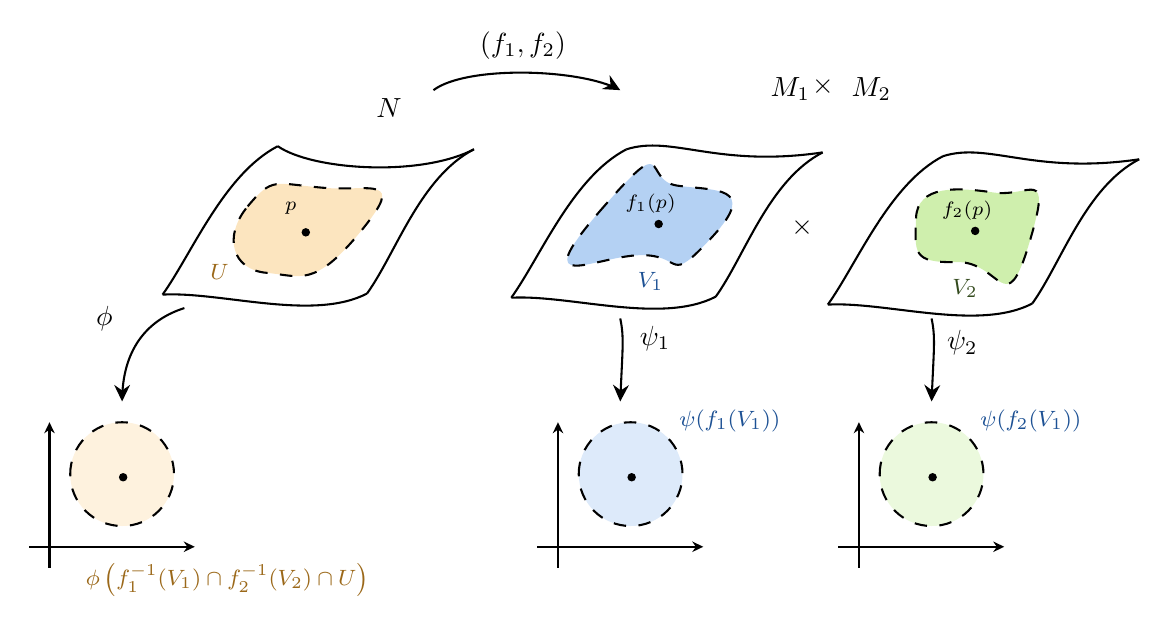
\begin{tikzpicture}[x=0.75pt,y=0.75pt,yscale=-1,xscale=1]
		%uncomment if require: \path (0,300); %set diagram left start at 0, and has height of 300
		
		%Curve Lines [id:da10777202147976128] 
		\draw    (89.5,138.5) .. controls (103.5,119) and (119,80.5) .. (145,67) ;
		%Curve Lines [id:da9226409814736687] 
		\draw    (89.5,138.5) .. controls (118,137) and (162,151.5) .. (188,138) ;
		%Curve Lines [id:da6153501766442295] 
		\draw    (188,138) .. controls (202,118.5) and (213.5,82) .. (239.5,68.5) ;
		%Curve Lines [id:da8299437341096081] 
		\draw    (145,67) .. controls (161.5,78.5) and (213.5,82) .. (239.5,68.5) ;
		%Curve Lines [id:da708998797665932] 
		\draw    (257.5,140) .. controls (271.5,120.5) and (287,82) .. (313,68.5) ;
		%Curve Lines [id:da5763078865113123] 
		\draw    (257.5,140) .. controls (286,138.5) and (330,153) .. (356,139.5) ;
		%Curve Lines [id:da17448723811544053] 
		\draw    (356,139.5) .. controls (370,120) and (381.5,83.5) .. (407.5,70) ;
		%Curve Lines [id:da5843329628503129] 
		\draw    (313,68.5) .. controls (335,61.5) and (356.5,77.5) .. (407.5,70) ;
		%Shape: Polygon Curved [id:ds719249129813768] 
		\draw  [fill={rgb, 255:red, 245; green, 166; blue, 35 }  ,fill opacity=0.29 ][dash pattern={on 4.5pt off 4.5pt}] (130.5,96) .. controls (142.5,81.5) and (143.5,85) .. (166.5,87) .. controls (189.5,89) and (207.5,80.5) .. (185,108) .. controls (162.5,135.5) and (156,129.5) .. (139.5,128) .. controls (123,126.5) and (118.5,110.5) .. (130.5,96) -- cycle ;
		%Shape: Polygon Curved [id:ds20297397591709365] 
		\draw  [fill={rgb, 255:red, 74; green, 144; blue, 226 }  ,fill opacity=0.41 ][dash pattern={on 4.5pt off 4.5pt}] (300,98.5) .. controls (335.5,57.5) and (320,83.5) .. (337.5,86) .. controls (355,88.5) and (377,86) .. (354.5,110.5) .. controls (332,135) and (341,119) .. (319.5,119.5) .. controls (298,120) and (264.5,139.5) .. (300,98.5) -- cycle ;
		%Straight Lines [id:da8177031700071737] 
		\draw    (35,203) -- (35,270) ;
		\draw [shift={(35,200)}, rotate = 90] [fill={rgb, 255:red, 0; green, 0; blue, 0 }  ][line width=0.08]  [draw opacity=0] (5.36,-2.57) -- (0,0) -- (5.36,2.57) -- (3.56,0) -- cycle    ;
		%Straight Lines [id:da5847590524068735] 
		\draw    (102,260) -- (25,260) ;
		\draw [shift={(105,260)}, rotate = 180] [fill={rgb, 255:red, 0; green, 0; blue, 0 }  ][line width=0.08]  [draw opacity=0] (5.36,-2.57) -- (0,0) -- (5.36,2.57) -- (3.56,0) -- cycle    ;
		%Shape: Circle [id:dp5757945587417739] 
		\draw  [fill={rgb, 255:red, 245; green, 166; blue, 35 }  ,fill opacity=0.15 ][dash pattern={on 4.5pt off 4.5pt}] (45,225) .. controls (45,211.19) and (56.19,200) .. (70,200) .. controls (83.81,200) and (95,211.19) .. (95,225) .. controls (95,238.81) and (83.81,250) .. (70,250) .. controls (56.19,250) and (45,238.81) .. (45,225) -- cycle ;
		%Straight Lines [id:da9243110317223102] 
		\draw    (280,203) -- (280,270) ;
		\draw [shift={(280,200)}, rotate = 90] [fill={rgb, 255:red, 0; green, 0; blue, 0 }  ][line width=0.08]  [draw opacity=0] (5.36,-2.57) -- (0,0) -- (5.36,2.57) -- (3.56,0) -- cycle    ;
		%Straight Lines [id:da35917271861832445] 
		\draw    (347,260) -- (270,260) ;
		\draw [shift={(350,260)}, rotate = 180] [fill={rgb, 255:red, 0; green, 0; blue, 0 }  ][line width=0.08]  [draw opacity=0] (5.36,-2.57) -- (0,0) -- (5.36,2.57) -- (3.56,0) -- cycle    ;
		%Shape: Circle [id:dp7567118959752777] 
		\draw  [fill={rgb, 255:red, 74; green, 144; blue, 226 }  ,fill opacity=0.19 ][dash pattern={on 4.5pt off 4.5pt}] (290,225) .. controls (290,211.19) and (301.19,200) .. (315,200) .. controls (328.81,200) and (340,211.19) .. (340,225) .. controls (340,238.81) and (328.81,250) .. (315,250) .. controls (301.19,250) and (290,238.81) .. (290,225) -- cycle ;
		%Curve Lines [id:da8387568355499948] 
		\draw    (220,40) .. controls (235.36,28.48) and (286.66,29.4) .. (307.55,38.78) ;
		\draw [shift={(310,40)}, rotate = 208.93] [fill={rgb, 255:red, 0; green, 0; blue, 0 }  ][line width=0.08]  [draw opacity=0] (8.04,-3.86) -- (0,0) -- (8.04,3.86) -- (5.34,0) -- cycle    ;
		%Curve Lines [id:da5596780294001671] 
		\draw    (310,150) .. controls (311.92,159.12) and (311.08,164.55) .. (310.12,187.09) ;
		\draw [shift={(310,190)}, rotate = 272.29] [fill={rgb, 255:red, 0; green, 0; blue, 0 }  ][line width=0.08]  [draw opacity=0] (8.04,-3.86) -- (0,0) -- (8.04,3.86) -- (5.34,0) -- cycle    ;
		%Curve Lines [id:da33319736118491083] 
		\draw    (100,145) .. controls (83.11,150.31) and (70.88,163.53) .. (70.05,187.36) ;
		\draw [shift={(70,190)}, rotate = 270] [fill={rgb, 255:red, 0; green, 0; blue, 0 }  ][line width=0.08]  [draw opacity=0] (8.04,-3.86) -- (0,0) -- (8.04,3.86) -- (5.34,0) -- cycle    ;
		%Shape: Circle [id:dp912491598557873] 
		\draw  [fill={rgb, 255:red, 0; green, 0; blue, 0 }  ,fill opacity=1 ] (157,108.5) .. controls (157,107.67) and (157.67,107) .. (158.5,107) .. controls (159.33,107) and (160,107.67) .. (160,108.5) .. controls (160,109.33) and (159.33,110) .. (158.5,110) .. controls (157.67,110) and (157,109.33) .. (157,108.5) -- cycle ;
		%Shape: Circle [id:dp5874182665613439] 
		\draw  [fill={rgb, 255:red, 0; green, 0; blue, 0 }  ,fill opacity=1 ] (327,104.5) .. controls (327,103.67) and (327.67,103) .. (328.5,103) .. controls (329.33,103) and (330,103.67) .. (330,104.5) .. controls (330,105.33) and (329.33,106) .. (328.5,106) .. controls (327.67,106) and (327,105.33) .. (327,104.5) -- cycle ;
		%Shape: Circle [id:dp6918787727605586] 
		\draw  [fill={rgb, 255:red, 0; green, 0; blue, 0 }  ,fill opacity=1 ] (69,226.5) .. controls (69,225.67) and (69.67,225) .. (70.5,225) .. controls (71.33,225) and (72,225.67) .. (72,226.5) .. controls (72,227.33) and (71.33,228) .. (70.5,228) .. controls (69.67,228) and (69,227.33) .. (69,226.5) -- cycle ;
		%Shape: Circle [id:dp5802827719353891] 
		\draw  [fill={rgb, 255:red, 0; green, 0; blue, 0 }  ,fill opacity=1 ] (314,226.5) .. controls (314,225.67) and (314.67,225) .. (315.5,225) .. controls (316.33,225) and (317,225.67) .. (317,226.5) .. controls (317,227.33) and (316.33,228) .. (315.5,228) .. controls (314.67,228) and (314,227.33) .. (314,226.5) -- cycle ;
		%Curve Lines [id:da5866172687533027] 
		\draw    (410,143.32) .. controls (424,123.82) and (439.5,85.32) .. (465.5,71.82) ;
		%Curve Lines [id:da33769380232352386] 
		\draw    (410,143.32) .. controls (438.5,141.82) and (482.5,156.32) .. (508.5,142.82) ;
		%Curve Lines [id:da5667601010223242] 
		\draw    (508.5,142.82) .. controls (522.5,123.32) and (534,86.82) .. (560,73.32) ;
		%Curve Lines [id:da7766245611502776] 
		\draw    (465.5,71.82) .. controls (487.5,64.82) and (509,80.82) .. (560,73.32) ;
		%Shape: Polygon Curved [id:ds9848033990053162] 
		\draw  [fill={rgb, 255:red, 126; green, 211; blue, 33 }  ,fill opacity=0.37 ][dash pattern={on 4.5pt off 4.5pt}] (452.5,101.82) .. controls (453,85.5) and (472.5,86.82) .. (490,89.32) .. controls (507.5,91.82) and (518.5,75.5) .. (507,113.82) .. controls (495.5,152.14) and (493.5,122.32) .. (472,122.82) .. controls (450.5,123.32) and (452,118.14) .. (452.5,101.82) -- cycle ;
		%Shape: Circle [id:dp8441479070293367] 
		\draw  [fill={rgb, 255:red, 0; green, 0; blue, 0 }  ,fill opacity=1 ] (479.5,107.82) .. controls (479.5,106.99) and (480.17,106.32) .. (481,106.32) .. controls (481.83,106.32) and (482.5,106.99) .. (482.5,107.82) .. controls (482.5,108.65) and (481.83,109.32) .. (481,109.32) .. controls (480.17,109.32) and (479.5,108.65) .. (479.5,107.82) -- cycle ;
		%Straight Lines [id:da4245600664130684] 
		\draw    (425,203) -- (425,270) ;
		\draw [shift={(425,200)}, rotate = 90] [fill={rgb, 255:red, 0; green, 0; blue, 0 }  ][line width=0.08]  [draw opacity=0] (5.36,-2.57) -- (0,0) -- (5.36,2.57) -- (3.56,0) -- cycle    ;
		%Straight Lines [id:da8383634096867163] 
		\draw    (492,260) -- (415,260) ;
		\draw [shift={(495,260)}, rotate = 180] [fill={rgb, 255:red, 0; green, 0; blue, 0 }  ][line width=0.08]  [draw opacity=0] (5.36,-2.57) -- (0,0) -- (5.36,2.57) -- (3.56,0) -- cycle    ;
		%Shape: Circle [id:dp032856070596776865] 
		\draw  [fill={rgb, 255:red, 184; green, 233; blue, 134 }  ,fill opacity=0.28 ][dash pattern={on 4.5pt off 4.5pt}] (435,225) .. controls (435,211.19) and (446.19,200) .. (460,200) .. controls (473.81,200) and (485,211.19) .. (485,225) .. controls (485,238.81) and (473.81,250) .. (460,250) .. controls (446.19,250) and (435,238.81) .. (435,225) -- cycle ;
		%Shape: Circle [id:dp2655157582176253] 
		\draw  [fill={rgb, 255:red, 0; green, 0; blue, 0 }  ,fill opacity=1 ] (459,226.5) .. controls (459,225.67) and (459.67,225) .. (460.5,225) .. controls (461.33,225) and (462,225.67) .. (462,226.5) .. controls (462,227.33) and (461.33,228) .. (460.5,228) .. controls (459.67,228) and (459,227.33) .. (459,226.5) -- cycle ;
		%Curve Lines [id:da36500972985566005] 
		\draw    (460,150) .. controls (461.92,159.12) and (461.08,164.55) .. (460.12,187.09) ;
		\draw [shift={(460,190)}, rotate = 272.29] [fill={rgb, 255:red, 0; green, 0; blue, 0 }  ][line width=0.08]  [draw opacity=0] (8.04,-3.86) -- (0,0) -- (8.04,3.86) -- (5.34,0) -- cycle    ;
		
		% Text Node
		\draw (191,42.4) node [anchor=north west][inner sep=0.75pt]    {$N$};
		% Text Node
		\draw (381,32.4) node [anchor=north west][inner sep=0.75pt]    {$M_{1}$};
		% Text Node
		\draw (241,10.4) node [anchor=north west][inner sep=0.75pt]    {$( f_{1} ,f_{2})$};
		% Text Node
		\draw (318,152.4) node [anchor=north west][inner sep=0.75pt]    {$\psi _{1}$};
		% Text Node
		\draw (56,142.4) node [anchor=north west][inner sep=0.75pt]    {$\phi $};
		% Text Node
		\draw (147,92.4) node [anchor=north west][inner sep=0.75pt]  [font=\scriptsize]  {$p$};
		% Text Node
		\draw (311,88.4) node [anchor=north west][inner sep=0.75pt]  [font=\scriptsize]  {$f_{1}( p)$};
		% Text Node
		\draw (111,122.4) node [anchor=north west][inner sep=0.75pt]  [font=\footnotesize,color={rgb, 255:red, 155; green, 104; blue, 25 }  ,opacity=1 ]  {$U$};
		% Text Node
		\draw (317,126.4) node [anchor=north west][inner sep=0.75pt]  [font=\footnotesize,color={rgb, 255:red, 29; green, 81; blue, 148 }  ,opacity=1 ]  {$V_{1}$};
		% Text Node
		\draw (337,192.4) node [anchor=north west][inner sep=0.75pt]  [font=\footnotesize,color={rgb, 255:red, 29; green, 81; blue, 148 }  ,opacity=1 ]  {$\psi ( f_{1}( V_{1}))$};
		% Text Node
		\draw (51,266.4) node [anchor=north west][inner sep=0.75pt]  [font=\footnotesize,color={rgb, 255:red, 155; green, 104; blue, 25 }  ,opacity=1 ]  {$\phi \left( f_{1}^{-1}( V_{1}) \cap f_{2}^{-1}( V_{2}) \cap U\right)$};
		% Text Node
		\draw (463.5,91.72) node [anchor=north west][inner sep=0.75pt]  [font=\scriptsize]  {$f_{2}( p)$};
		% Text Node
		\draw (468.5,129.72) node [anchor=north west][inner sep=0.75pt]  [font=\footnotesize,color={rgb, 255:red, 52; green, 75; blue, 30 }  ,opacity=1 ]  {$V_{2}$};
		% Text Node
		\draw (482,192.4) node [anchor=north west][inner sep=0.75pt]  [font=\footnotesize,color={rgb, 255:red, 29; green, 81; blue, 148 }  ,opacity=1 ]  {$\psi ( f_{2}( V_{1}))$};
		% Text Node
		\draw (420,32.4) node [anchor=north west][inner sep=0.75pt]    {$M_{2}$};
		% Text Node
		\draw (391,100.4) node [anchor=north west][inner sep=0.75pt]    {$\times $};
		% Text Node
		\draw (466,154.4) node [anchor=north west][inner sep=0.75pt]    {$\psi _{2}$};
		% Text Node
		\draw (401,32.4) node [anchor=north west][inner sep=0.75pt]    {$\times $};
		
		
	\end{tikzpicture}
\end{figure}
	\FloatBarrier
	
	For the first direction, we will show that smoothness of $ (f_1,f_2): N \to M_1\times M_2 $ implies the smoothness of $ f_1:N\to M_1 $ and $ f_2: N \to M_2 $. As depicted in the picture above, let $ \phi $ be a coordinate map for $ N $ and $ \psi_1, \psi_2 $ be coordinate maps for $ M_1,M_2 $ respectively. Since $ (f_1,f_2) $ is smooth, then $ (\psi_1 \times \psi_2) \circ (f_1,f_2) $ is smooth. Let $ p \in N $, then
	\[ ((\psi_1 \times \psi_2) \circ (f_1,f_2) \circ \inv{\phi})(\phi(p)) =
	((\psi_1 \times \psi_2) \circ (f_1,f_2)) (p) = (\psi_1\times \psi_2)(f_1(p),f_2(p)) = (\psi_1(f_1(p)), \psi_2(f_2(p))).
	 \]
	This is a smooth map from $ \R^n $ to $ \R^{m_1+m_2} $. Thus the components of the function are also smooth.
	
	For the converse, we need to show that the smoothness of $ f_1 $ and $ f_2 $ implies the smoothness of $ (f_1,f_2) $. Similar to the argument above, the smoothness of $ (f_1,f_2) $ follows immediately from the smoothness of the components.
\end{solution}

\begin{problem}[Smooth functions on unit circle (W. Tu)]
	We have studied before that the unit circle $ S^1 $ defined by $ x^2 + y^2 = 1 $ in $ \R^2 $ is a $ C^\infty $ manifold. Prove that a smooth function $ f: \R^2 \to \R $ defined on $ \R^2 $ restricts to a $ C^\infty $ function on $ S^1 $.
\end{problem}

\begin{solution}
	Consider the following inclusion map
	\[ i: S^1 \to \R^2 \]
	defined as $ i(p) = (x(p),y(p)) $, where $ x,y $ are the standard coordinate functions. The restriction of $ f $ to manifold will be
	\[ f|_{S^1} = f \circ i. \]
	To show that $ f|_{S^1} $ is smooth, we just need to show that the inclusion map is smooth. To show this we need to show that the components of this vector valued function is smooth. We start by showing that $ x $ is smooth. We use the same charts as in \autoref{problem:S^1Charts}. Let $ p \in S^1 $. If $ p \in U_3 \cap U_4 $ then we have
	\[ \mathds{1}_{(0,1)}\circ x \circ \inv{\phi_3} = \mathds{1}_{(0,1)}: (-1,1) \to \R^2, \qquad \mathds{1}_{(0,1)}\circ x \circ \inv{\phi_4} = \mathds{1}_{(0,1)}: (-1,1) \to \R^2,  \]
	which are both identity maps, thus smooth. So $  x $ is smooth on $ U_3\cap U_4 $. For $ U_1 $ we have
	\[ \mathds{1}_{(0,1)}\circ x \circ \inv{\phi_1}(x) = -\sqrt{1-x^2}, \qquad\text{for } x \in \phi_1(U_1) = (-1,1) \]
	thus $ x $ is smooth on $ U_1 $ as well. For $ U_2 $ we have
	\[ \mathds{1}_{(0,1)}\circ x \circ \inv{\phi_2}(x) = \sqrt{1-x^2}, \qquad\text{for } x \in \phi_2(U_2) = (-1,1) \]
	thus $  x $ is smooth on $ U_2  $ as well. We can use a similar strategy to show that the coordinate function $ y $ is also smooth.
\end{solution}



\begin{problem}
	The general linear group $ \operatorname{GL}(n,\R) $ is the set of all real valued matrices with non-zero determinant under matrix multiplication. In other words
	\[ \operatorname{GL}(n,\R) = \set{A = \left[ a_{ij} \right] \in \R^{n\times n}\ |\ \det(A) \neq 0} . \]
	We can see this as an open subset of $ \R^{n\times n} $, thus it is a manifold. Show that this forms a Lie group.
\end{problem}

\begin{solution}
	Let $ A,B $ be two matrices in the manifold. Then the $ i,j $ element of $ AB $ is
	\[ (AB)_{ij} = \sum_{k=1}^{n} A_{ik}B_{kj} \]
	which is a polynomial in the coordinates of $ A $ and $ B $, thus it is smooth. To show that the inverse is also smooth, for any function $ A $ in the manifold we have
	\[ \inv{A} = \frac{1}{\det(A)} \cdot (-1)^{i+j}((i,j)\text{- minor of $ A $}). \]
	The $ (i,j)\text{-minor} $ of matrix $ A $ is the determinant of the sub matrix by deleting the $ i\text{-th} $ row and $ j\text{th} $ column, which is again a polynomial in the coordinates of $ A $ and $ B $, thus smooth (given that $ \det(A) \neq 0 $).
\end{solution}

\begin{problem}[Jacobian matrix os a transition map (form W. Tu)]
	Let $ (U,\phi) = (U,x^1,\cdots,x^n) $ and $ (V,\psi) = (V,y^1,\cdots,y^n) $ be overlapping charts on a manifold $ M $. The transition map $ \psi \circ\inv{\phi}: \phi(U\cap V) \to \psi(U\cap V) $ is a diffeomorphism of open subsets of $ \R^n $. Show that its Jacobian matrix $ J(\psi\circ\inv{\phi}) $ at $ \phi(p) $ is the matrix $ [\partial y^i/\partial x^j] $ of partial derivatives at $ p $.
\end{problem}
\begin{solution}
	From the definition of the Jacobian matrix we can write
	\[ J(\psi \circ \inv{\phi}) = \frac{\partial (\psi \circ \inv{\phi})^i}{\partial r^j} =  \frac{\partial (r^i \circ \psi \circ \inv{\phi})}{\partial r^j} = \frac{\partial (y^i \circ \inv{\phi})}{\partial r^j} = \frac{\partial y^i}{\partial x^j}. \]
\end{solution}

\begin{observation}[Some mnemonics for the Jacobian matrix]
	Here I introduce a symbolic mnemonic of remembering the form of the Jacobian matrix of a smooth map between manifolds. Let $ F:N\to M $ a smooth map between manifolds. Since this function is from $ N $ to $ M $, then the Jacobian matrix will be of the form
	\[ J(F) = [\partial F^i / \partial x^j] \] 
	where $ x^j $ a local coordinate in $ N $ and $ F^i = y^i \circ F $ where $ y^i $ is a local coordinate in $ M $. What we mean by local coordinates here is that for a point $ p $ on the manifold for which we want to calculate the Jacobian matrix, there are charts $ (U,x^1\cdots,x^n) $ and $ (V,y^1,\cdots,y^n) $ on $ N $ and $ M $ respectively such that $ p \in U $ and $ F(U) \subset V $.
	
	As another example, in the question above, since the function $ \psi\circ\inv{\phi} $ is defined from $ \R^n \to \R^n $, then the Jacobian of this function starts with coordinates of $ \R^n $, i.e. $ r^i $.
\end{observation}

\begin{problem}[From W. Tu]
	Find all points in $ \R^2 $ in a neighborhood of which the functions given by $ x^2 + y^2 -1  $ and $ y $ can serve as a local coordinate system.
\end{problem}
\begin{solution}
	Define $ F^1(x,y) = x^2 + y^2 -1 $ and $ F^2(x,y) = y  $. Then the pair $ (F^1,F^2) $ is locally invertible, thus can serve as a local diffeomorphism to $ \R^2 $, thus a coordinate map if the Jacobian determinant $ [\partial F^i /\partial x^i] $ is not zero. I.e.
	\[ \det\matt{2x}{2y}{0}{1} = 2x \neq 0 \implies x \neq 0. \]
	Thus the function $ F = (F^1,F^2) $ can act as a local coordinate map everywhere except for on the points on the $ y $ axis. You can see why this happens in the plots below. As you can see, any path that is not crossing the $ y $ axis with zero vertical velocity is diffeormorphically mapped to an smooth curve. But when the curve passes through the $ y $ axis with a zero vertical velocity, then the curve folds on itself when mapped by $ F $, thus $ F $ fails be locally invertible and thus fails to be a coordinate map. Thus for any point that is not on the $ y $ axis, we can find an open set small enough that does not overlap with the $ y $ axis. But there is no such an open ball for the points on the $ y $ axis.	You can try the online plotting tool that I have configured to generate the following plots \href{https://www.desmos.com/calculator/pam0whmnbs}{here}.
	\begin{figure}[h!]
		\centering
		\includegraphics[width=0.8\linewidth]{Images/diffeomorphismExample}
	\end{figure}
	
\end{solution}

\begin{problem}[Differentiable structure on $ \R $]
	Let $ \R $ be the real line with the differentiable structure given by the maximal atlas of the chart $ (\R, \phi=\mathds{1}:\R \to \R) $, and let $ \R' $ be the real line with the differentiable structure given by the maxima atlas of the chart $ (\R, \psi:\R\to\R) $, where $ \psi(x) = x^{1/3} $.
	\begin{enumerate}[(a)]
		\item Show that these two differentiable structures are distinct.
		\item Show that there is a diffeomorphism between $ \R $ and $ \R' $. (\emph{Hint:} The identity map $ \R \to \R  $ is not  the desired diffeomorphism; in fact, this map is not smooth).
	\end{enumerate}
\end{problem}
\begin{solution}
	\begin{enumerate}[(a)]
		\item Let $ M_1 $ be the atlas containing $ (\R,\phi) $ and $ M_2 $ the atlas containing $ (\R,\psi) $. Assume $ M_1 = M_2 $. Then $ (\R,\phi) $ should be compatible with $ (\R,\psi) $, i.e. the functions
		\[ \psi \circ \inv{\phi} = \R \to \R, \qquad \phi\circ \inv{\psi}:\R \to \R, \]
		are smooth. This is not true since $ (\psi \circ \inv{\phi} )(x) = x^{1/3} $ that is not differentiable at $ x=0 $. So $ M_1 \neq M_2 $ and these two atlases are distinct.
		\item For a more clear demonstration, the manifold with atlas generated by $ (\R,\phi=\mathds{1}:\R\to \R) $ the manifold $ R $, and call the other manifold the manifold $ R' $. Define the map $ F $ between manifolds
		\[ F: R \to R' \]
		as $ F(p) = p^3 $ for $ p \in R $. The inverse of this map will be $ \inv{F}(p) = p^{1/3} $. To show this map is a diffeomorphism, we need to show that the following 
		\[ \psi \circ F \circ \inv{\phi}: \phi(U)\to \psi(F(U)), \qquad \phi\circ\inv{F}\circ\inv{\phi}: \phi(V) \to \phi(\inv{F}(V)), \]
		are smooth. In  equations above, $ (U,\phi: x\mapsto x) $ is some coordinate system (i.e. chart) on $ R $ whereas $ (V,\psi: x\mapsto x^1/3) $ is a coordinate system on $ R' $. Let $ \phi(x) = x \in \phi(U\cap V) $. Then
		\[ (\psi\circ F \circ\inv{\phi})(x) = \psi(F(x)) = \psi(x^3) = x,\]
		which is the identity map and is smooth. Furthermore
		\[( \phi\circ\inv{F}\circ\inv{\phi})(x) = \phi(F^{-1}(x^3)) = \psi(x) = x,\]
		which is again the identity map and is smooth. Thus the map $ F $ is a diffeomorphism between the manifolds.
	\end{enumerate}
\end{solution}


\begin{problem}[The smoothness of an inclusion map (From L. Tu)]
	Let $ M $ and $ N $ be manifolds and let $ q_0 $ be a point in $ N $. Prove that the inclusion map $ i_{q_0}: M \to M\times N $, $ i_{q_0}(p) = (p,q_0) $, is $ C^\infty $.
\end{problem}
